\section{Impact of pile-up}

\label{sec:pileup}

The main limitation of our analysis so far is the fact that
pile-up (PU) effects have not been accounted for
not accounted for.
%
However, any realistic feasibility study at the HL-LHC, specially
one 
such the present that relies on the careful modeling
of kinematic distributions,
requires assessing the robustness of the conclusions
with respect to the inclusion of PU.
%
In this section, we show how our qualitative results, in particular
the enhanced signal significance provided by the MVA, are robust
in the presence of  PU.


First of all, we describe the simulation of the 
PU conditions  expected at the HL-LHC, and discuss the settings of
the PU subtraction strategy that we adopt.
%
Then we present the validation of the PU subtraction,
and compare a number of distributions, including substructure variables,
with and without PU.
%
Finally we revisit the MVA analysis of Sect.~\ref{sec:mva}, and
show that our qualitative conclusions are robust
in the presence of realistic PU conditions, finding
a combined
signal significance of $S/\sqrt{B}\simeq 4$.


\subsection{PU subtraction with {\tt SoftKiller}}

To study the impact of PU in our analysis,
Minimum Bias (MB) events,
including Multiple Parton Interactions (MPI), have been generated
with {\tt Pythia8}, and
superimposed to the signal
and background samples described in Sect.~\ref{mcgeneration}.
%
We have explored two scenarios for the amount of PU expected
at the HL-LHC, one with a mean number of
PU vertices per bunch crossing of $\la n_{\rm PU}\ra=80$, and another
with $\la n_{\rm PU}\ra=150$.
%
In order to subtract the PU, a number of techniques
have been developed
recently~\cite{Cacciari:2009dp,TheATLAScollaboration:2013pia,Butterworth:2008iy,Cacciari:2007fd,Krohn:2009th,Krohn:2013lba,Ellis:2009me,Bertolini:2014bba,Cacciari:2014gra,Cacciari:2014jta,Berta:2014eza,Larkoski:2014wba}.\footnote{
These techniques have also important applications in the subtraction
of the UE/MPI contamination for jet reconstruction
in heavy ion collisions~\cite{Cacciari:2010te}.
}
%
In this work, PU  will be subtracted by means
of the the {\tt SoftKiller} (SK)
method~\cite{Cacciari:2014gra}, as implemented in {\tt FastJet}.
%

The idea underlying {\tt SoftKiller} is based on eliminating particles
below a given cut-off in their transverse momentum, $p_T^{\rm (cut)}$, whose
value is dynamically determined in a way that makes the event-wide
transverse-momentum flow density $\rho$ vanish.
%
This $p_T$ flow density is defined as
\be
\rho\equiv{\rm median}_i \Bigg\{ \frac{p_{Ti}}{A_i}\Bigg\} \, ,
\ee
where the median is computed over all the patches $i$ with area
$A_i$ and transverse momentum $p_{Ti}$ in which the $\lp \eta,\phi\rp$ plane
is partitioned.
%
From its definition in terms of the median,
we observe that the value of $p_T^{(\rm cut)}$
will be dynamically raised until half of the patches have $\rho=0$.
%
The size and number of these patches is a free parameter of the algorithm -
here we will use square patches with length $a=0.4$.
%
We restrict ourselves to the central rapidity region,
$|\eta| \le 2.5$, for the estimation of the
$p_T$ flow density $\rho$.
%
In this analysis, {\tt SoftKiller} method is applied
to particles at the end of the parton shower, before
jet clustering.

To validate PU subtraction,
we now compare different kinematical distributions
in the case without PU and in the case
with PU subtracted with {\tt SoftKiller}.
%
Then we will also compare some specific distributions
also in the case where PU has not been subtracted.
%
We find that
{\tt SoftKiller} exhibits a reasonable
performance for the PU subtraction.
%
We  also obtain that the boosted category is less affected
by PU than the resolved category, as expected from the higher
$p_T$ threshold in the corresponding selection cuts.


First of all, let us validate both the implementation of our
simulation of PU, as well as the SK subtraction, by comparing the
invariant mass distributions of Higgs candidates in signal
events in the resolved category.
%
In Fig.~\ref{fig:PUvalidation} we show three curves: without PU,
with PU $\la n_{PU}\ra=80$ but without any subtraction, and the
same but now with the SK subtraction.
%
As expected, if PU is not subtracted there is a large shift in the Higgs mass
peak, by about 40 GeV.
%
Once SK subtraction is performed, we recover a distribution much closer
to the original ones, with only a small shift of $\simeq 5$ GeV in the mass
distribution.
%
As we will see below, the performance of SK is even better in the boosted category,
since the effects of PU are mitigated for high $p_T$ jets.

%%%%%%%%%%%%%%%%%%%%%%%%
\begin{figure}[t]
  \begin{center}
  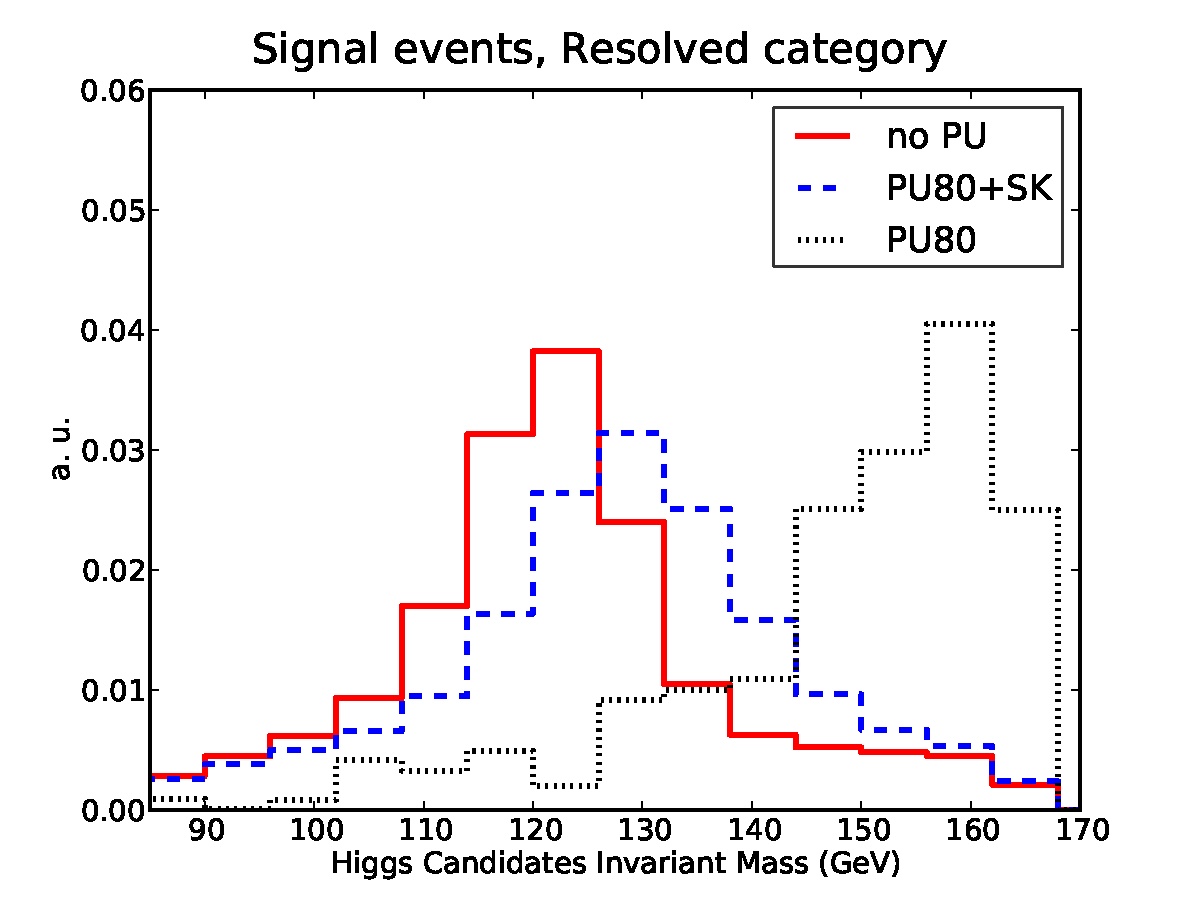
\includegraphics[width=0.68\textwidth]{plots/m_htot_res_signal_PUnoSK.pdf}
    \caption{\small
    The invariant mass distributions of Higgs candidates in signal
events, in the resolved category, comparing the results without PU,
with PU $\la n_{PU}\ra=80$ but without any subtraction, and the
corresponding results now with SK subtraction.
}
\label{fig:PUvalidation}
\end{center}
\end{figure}
%%%%%%%%%%%%%%%%%%%%%%%

Next, we compare more
 signal distributions with
and without PU, with $\la n_{\rm PU}\ra=80$ in the
former
case (and SK subtraction).
%
In Fig.~\ref{fig:m_H_PU} we show the invariant mass distribution
of the leading and subleading Higgs candidates, corresponding to both
the boosted
and resolved categories.
%
These distributions are plotted after the $b$-tagging, that is,
before they are used as input to the MVA.
%
As we can see, in the boosted category, the residual effects of PU
after the {\tt SoftKiller} subtraction are rather mild,
with the position of the Higgs mass peaks essentially
unchanged, and only a moderate distortion of the
distribution found.
%
The effects are more important for the resolved category, where PU
shifts the Higgs peak by an amount $\Delta m_h \simeq 5$ GeV.

%%%%%%%%%%%%%%%%%%%%%%%%
\begin{figure}[t]
  \begin{center}
      \vspace{-1cm}
      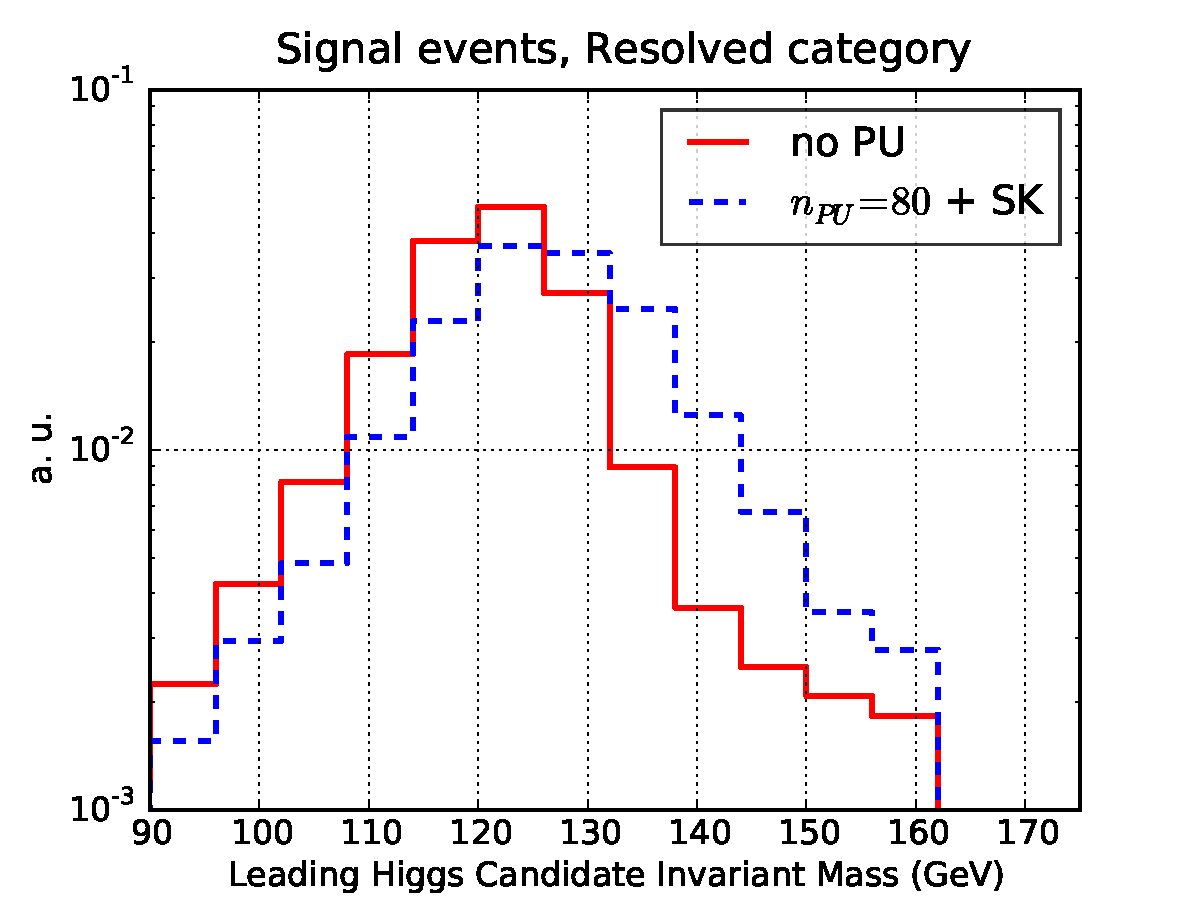
\includegraphics[width=0.49\textwidth]{plots/m_H0_res_comp.pdf}
      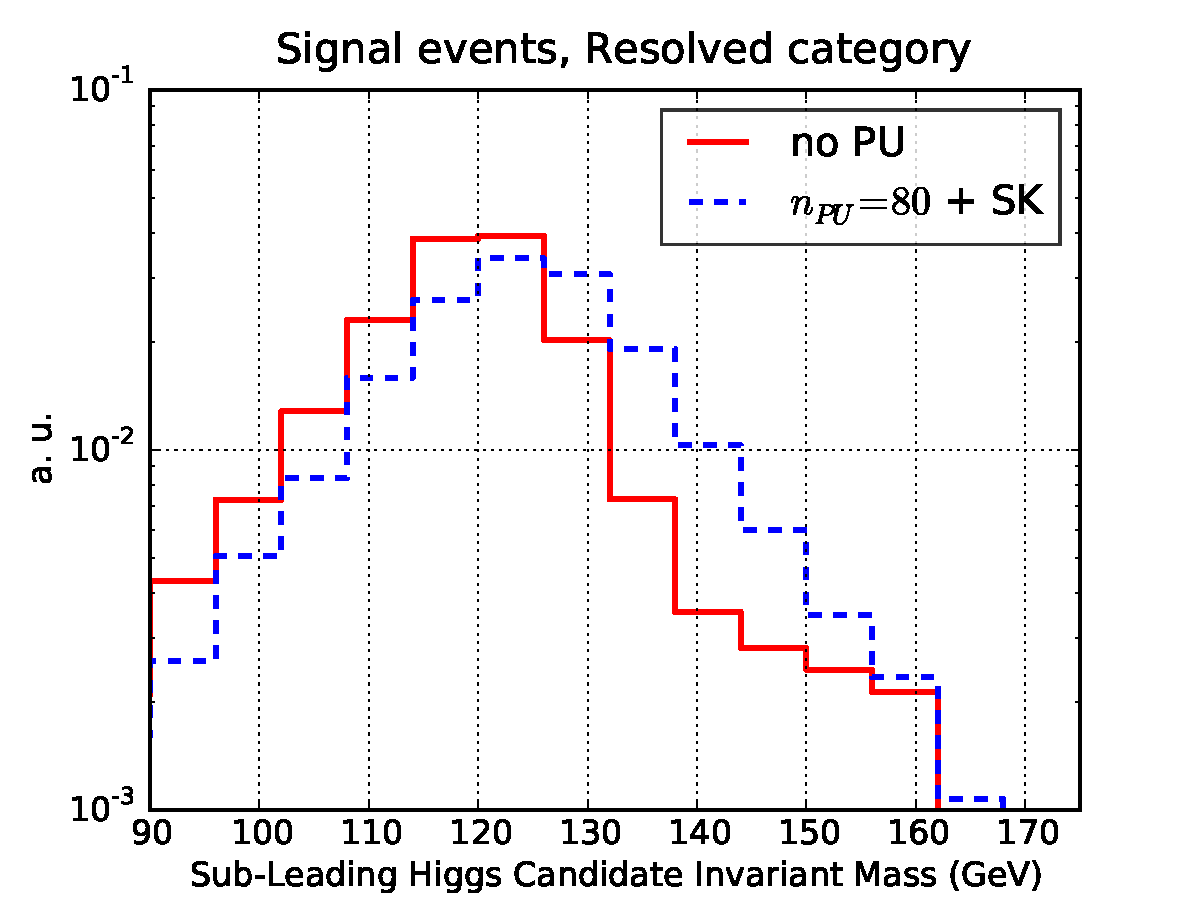
\includegraphics[width=0.49\textwidth]{plots/m_H1_res_comp.pdf}
      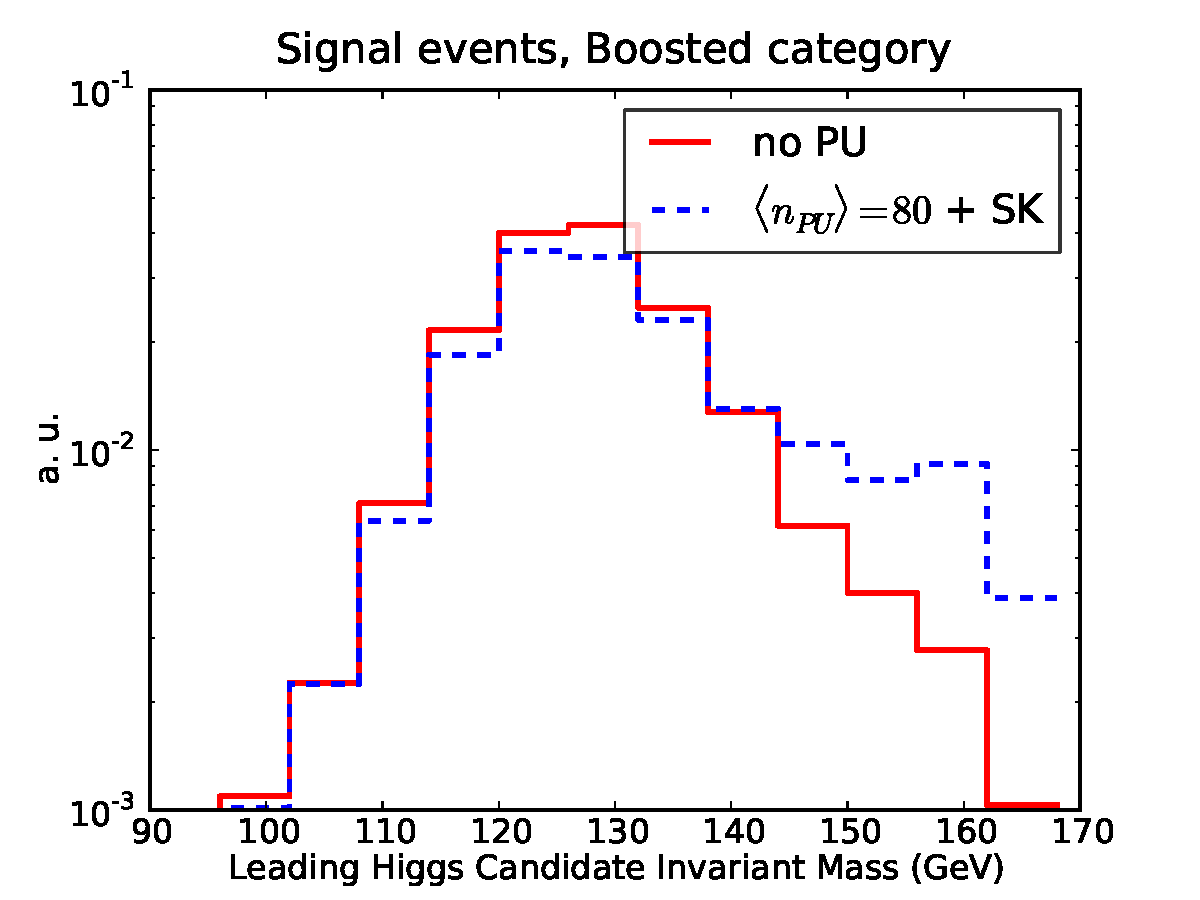
\includegraphics[width=0.49\textwidth]{plots/m_H0_bst_comp.pdf}
      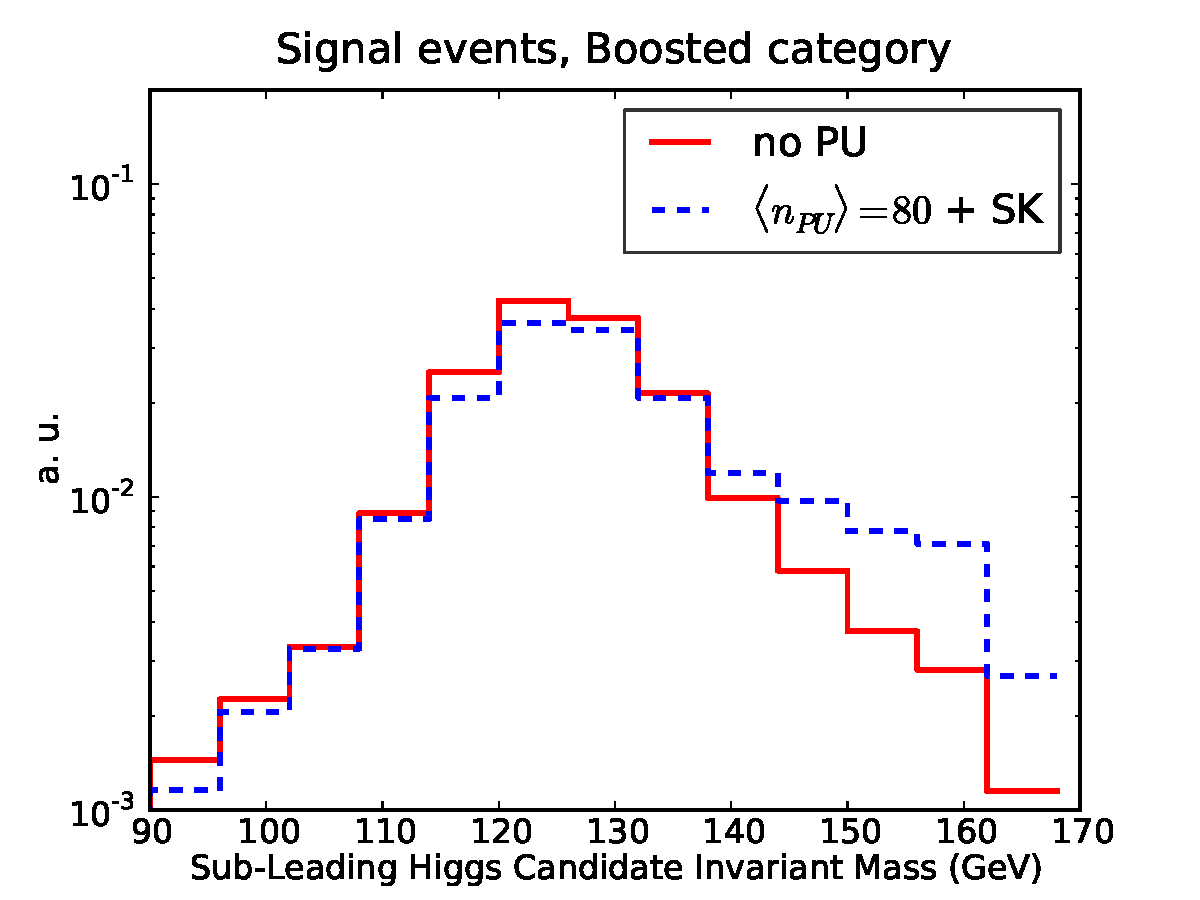
\includegraphics[width=0.49\textwidth]{plots/m_H1_bst_comp.pdf}
  \caption{\small
    Comparison of the invariant mass distributions of the leading (left plots)
    and subleading (right plots) Higgs candidates in the resolved
    (upper plots) and boosted (lower plots) categories,
    both without PU and with
    PU, $\la n_{PU}\ra=80$, subtracted with {\tt SoftKiller}.
}
\label{fig:m_H_PU}
\end{center}
\end{figure}
%%%%%%%%%%%%%%%%%%%%%%%

Next we compare the transverse momentum of the leading Higgs
candidate, $p_t^{h_1}$ and the invariant mass of the di-Higgs system
$m_{hh}$, in Fig.~\ref{fig:mHH_PU}, both for the boosted and
for the resolved categories.
%
In the case of the $p_T$ distribution, the differences between the selection
criteria for the resolved
and boosted categories is reflected in the rightward shift of the latter.
%
The effect of PU is negligible in the boosted case, and small
in the resolved case, except for large $p_T$ values.
%
For the case of the $m_{hh}$ distribution, similar conclusions
apply.
%
These comparisons validate the PU subtraction strategy
adopted in this work.


%%%%%%%%%%%%%%%%%%%%%%%%
\begin{figure}[t]
  \begin{center}
    \vspace{-1cm}
  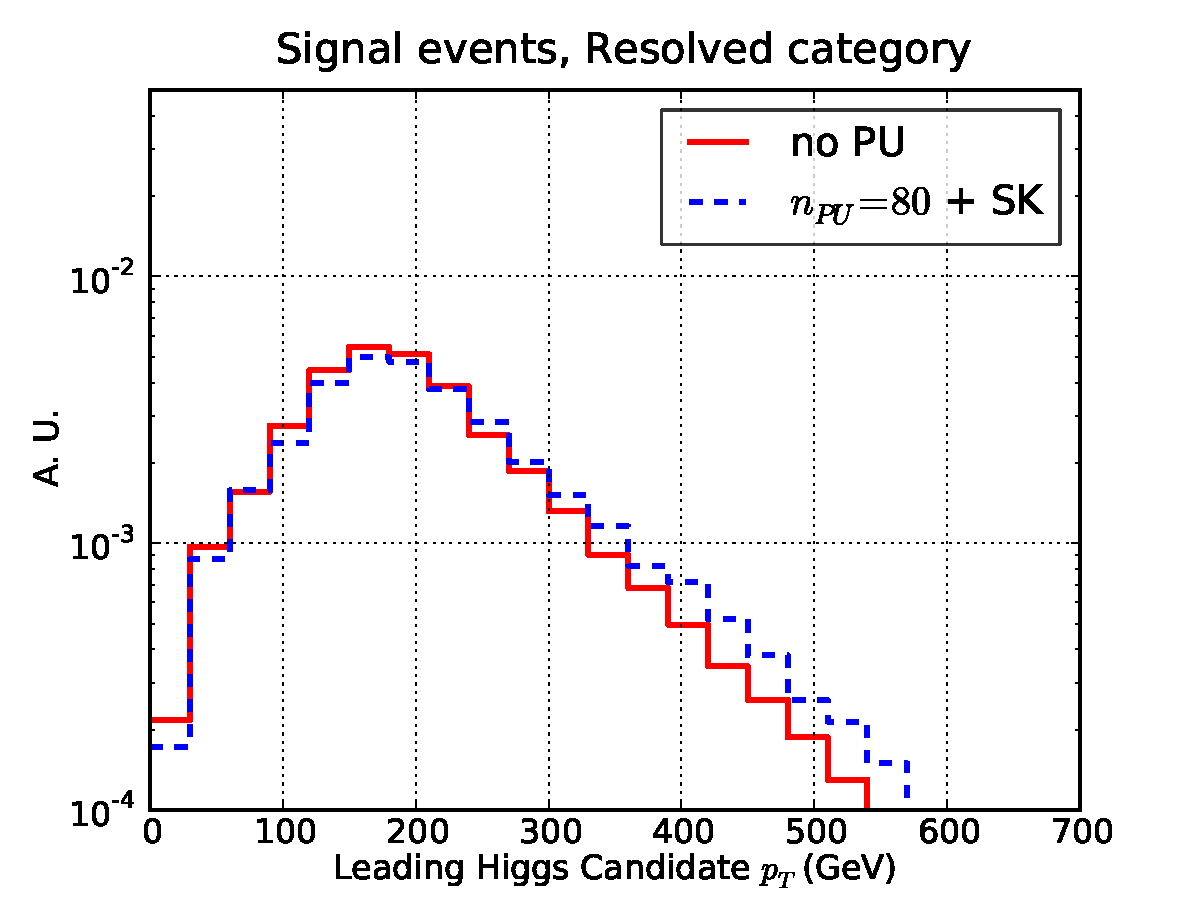
\includegraphics[width=0.49\textwidth]{plots/pt_H0_C2_res_comp.pdf}
  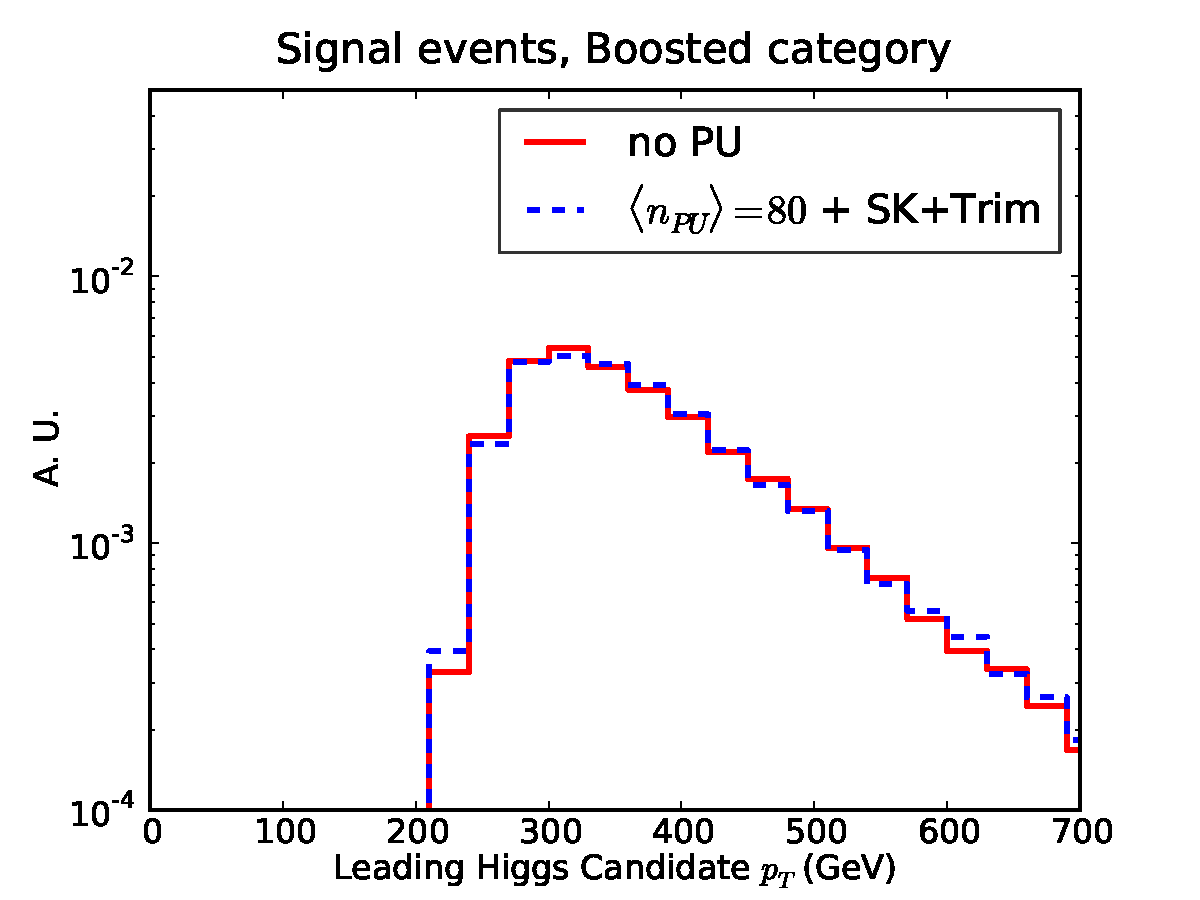
\includegraphics[width=0.49\textwidth]{plots/pt_H0_C2_bst_comp.pdf}
  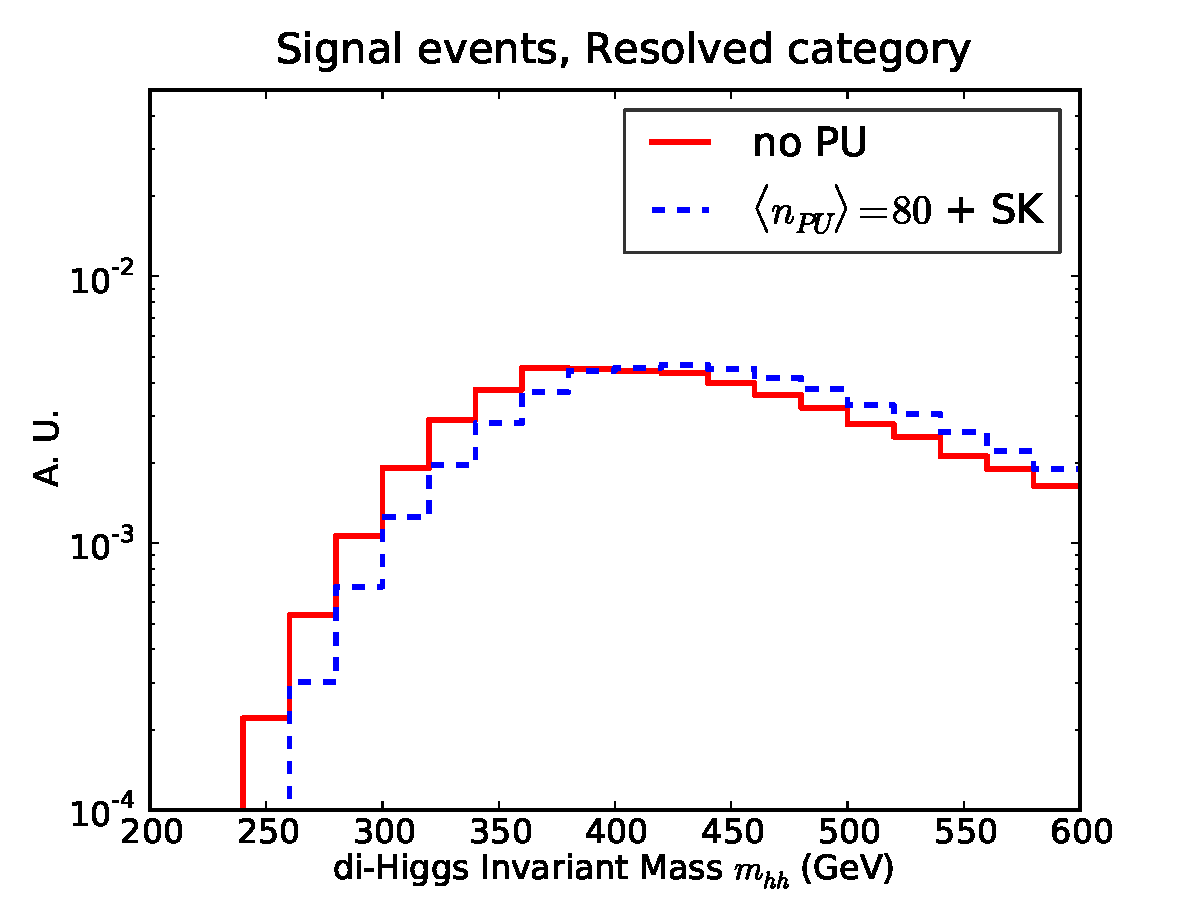
\includegraphics[width=0.49\textwidth]{plots/m_HH_C2_res_comp.pdf}
  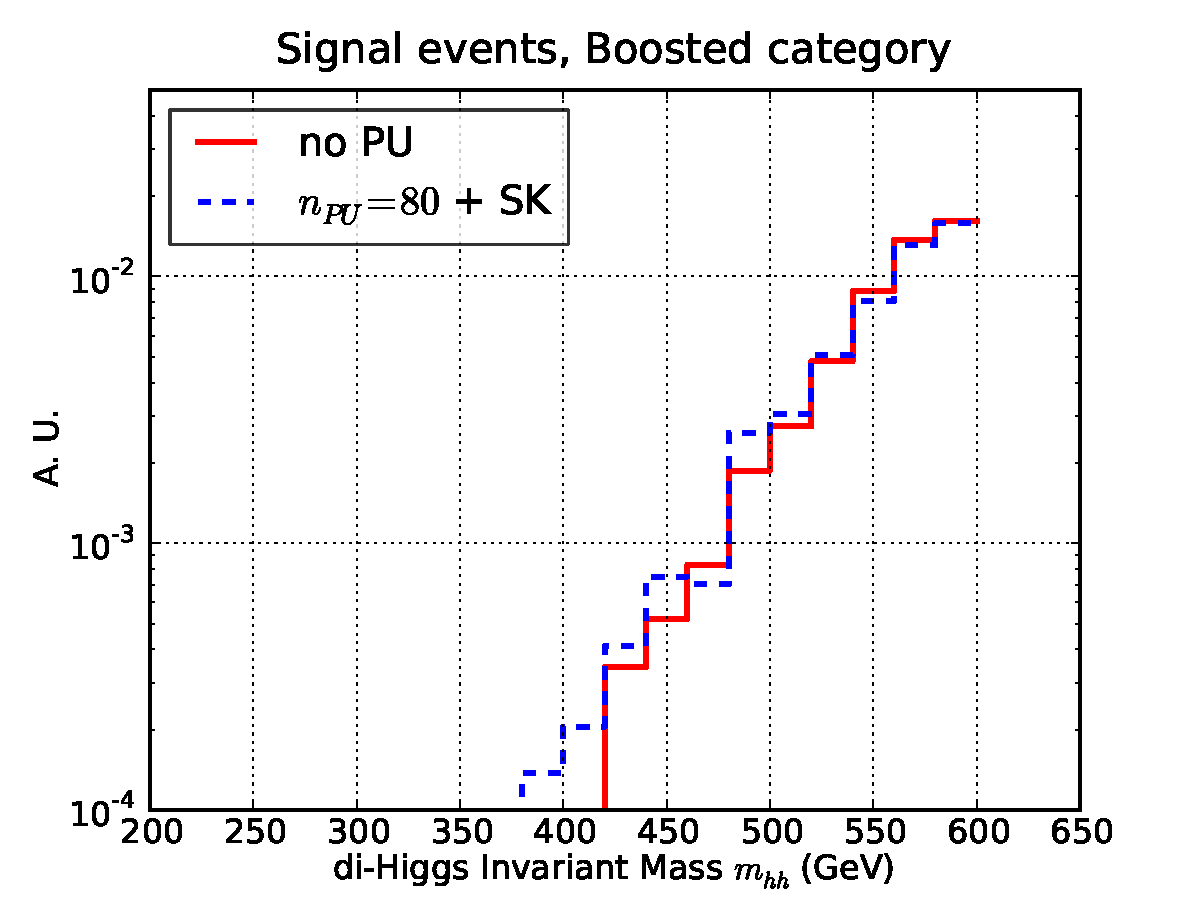
\includegraphics[width=0.49\textwidth]{plots/m_HH_C2_bst_comp.pdf}
  \caption{\small
    Comparison of the transverse momentum $p_T^h$ of the leading
    Higgs candidate (upper plots) and of the invariant mass $m_{hh}$
    of the di-Higgs system (lower plots) in the resolved
    (left plots) and boosted (right plots) categories,
    without PU and with $\la n_{PU}\ra=80$ subtracted with {\tt SoftKiller}.
}
\label{fig:mHH_PU}
\end{center}
\end{figure}
%%%%%%%%%%%%%%%%%%%%%%%

We can also assess the impact of PU in representative
substructure variables
used as input to the MVA in the boosted category.
%
In particular we consider the subjetiness variable,
$\tau_{21}$, Eq.~(\ref{eq:tau21}), and the ratio
of energy correlation functions, $D_2^{(\beta)}$,
Eq.~(\ref{eq:d2}),
corresponding to the leading Higgs candidate.
%
This comparison is illustrated in Fig.~\ref{fig:Substructure_PU}.
%
As can be seen, these substructure variables, which
as demonstrated before carry a substantial
discrimination power, are relatively unaffected by PU.
%
Recall that the $D_2^{(\beta)}$ variable is
explicitly constructed~\cite{Larkoski:2013eya}
to be resilient
with respect to PU contamination.
%
Therefore, we do not expect a major loss of discrimination
power due to PU effects in our analysis.
%

%%%%%%%%%%%%%%%%%%%%%%%%
\begin{figure}[t]
  \begin{center}
  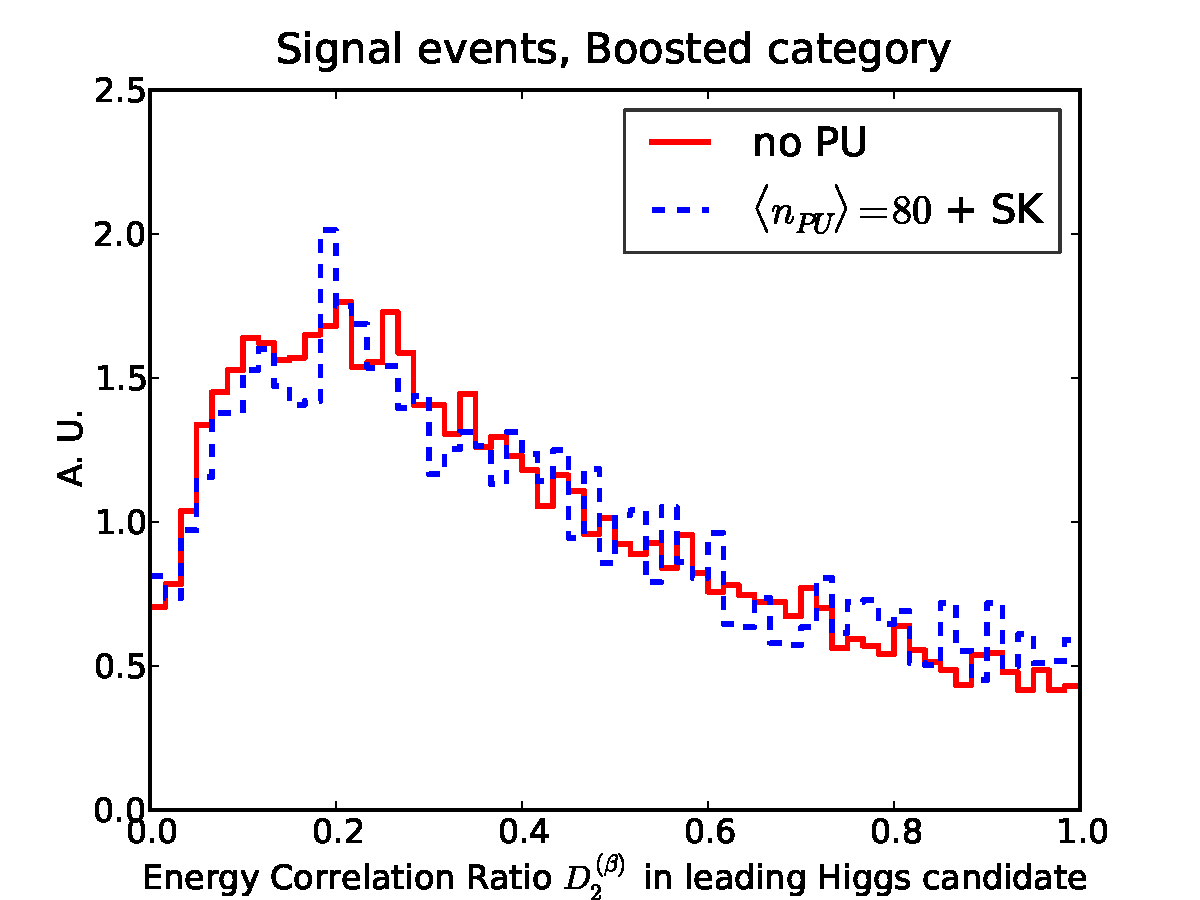
\includegraphics[width=0.49\textwidth]{plots/D2_h0_bst_comp.pdf}
  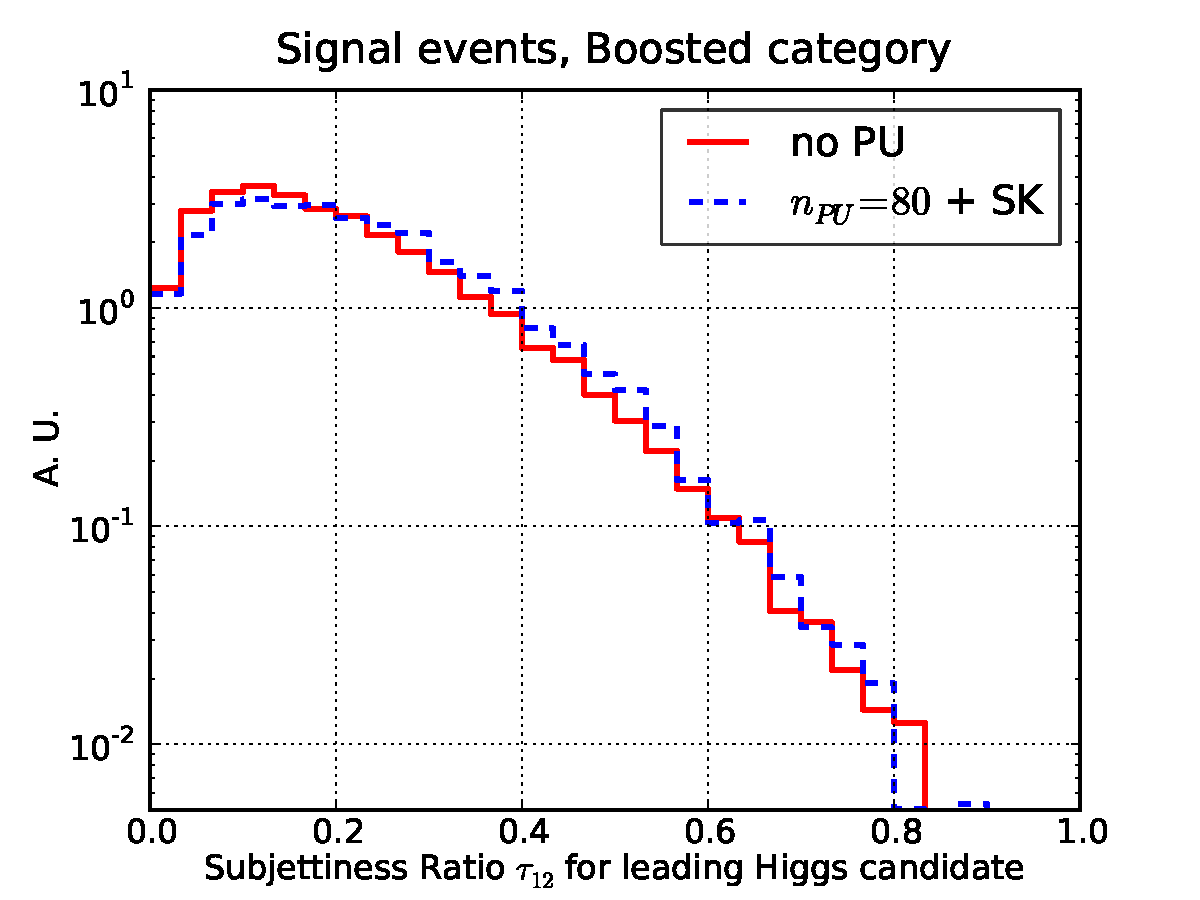
\includegraphics[width=0.49\textwidth]{plots/tau21_h0_bst_comp.pdf}
   \caption{\small
     Comparison of the substructure variables $D_2^{(\beta)}$ (left)
     and $\tau_{21}$ (right)
     for the leading Higgs candidate in the boosted category,
   without PU and with $\la n_{PU}\ra=80$ subtracted with {\tt SoftKiller}.
}
\label{fig:Substructure_PU}
\end{center}
\end{figure}
%%%%%%%%%%%%%%%%%%%%%%%

It is also interesting to quantify how
the relative differences between
signal over background distributions are affected in 
the presence of PU.
%
Considering first of all the boosted category,
in Fig.~\ref{fig:signal-vs-back-boosted} we compare
various kinematical distributions for signal and background events,
     with and without PU: the invariant mass, the $p_T$,
     the 2-jettiness $\tau_{21}$, and $\sqrt{d_{12}}$,
     the $k_T$ splitting scale, Eq.~(\ref{eq:ktsplitting}),
     all corresponding to
     the leading Higgs candidate.
     %
      We observe that the most of the relevant
      qualitative differences between signal
      and background distributions are maintained in the presence of PU.
      %
      This is specially clear for the substructure variables, which
      show a similar discrimination power both with and without
      PU.
     

%%%%%%%%%%%%%%%%%%%%%%%%
\begin{figure}[t]
  \begin{center}
  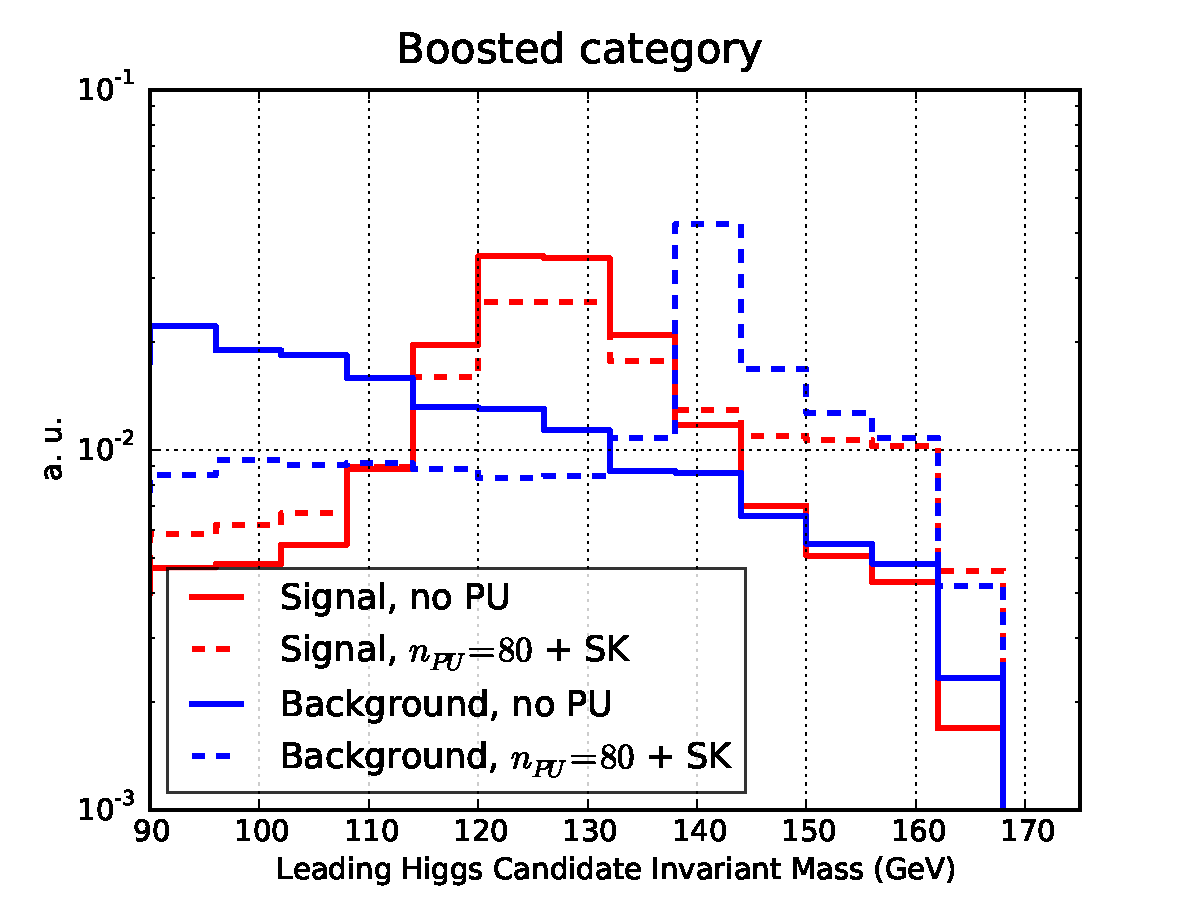
\includegraphics[width=0.49\textwidth]{plots/m_h0_bst_comp_back.pdf}
  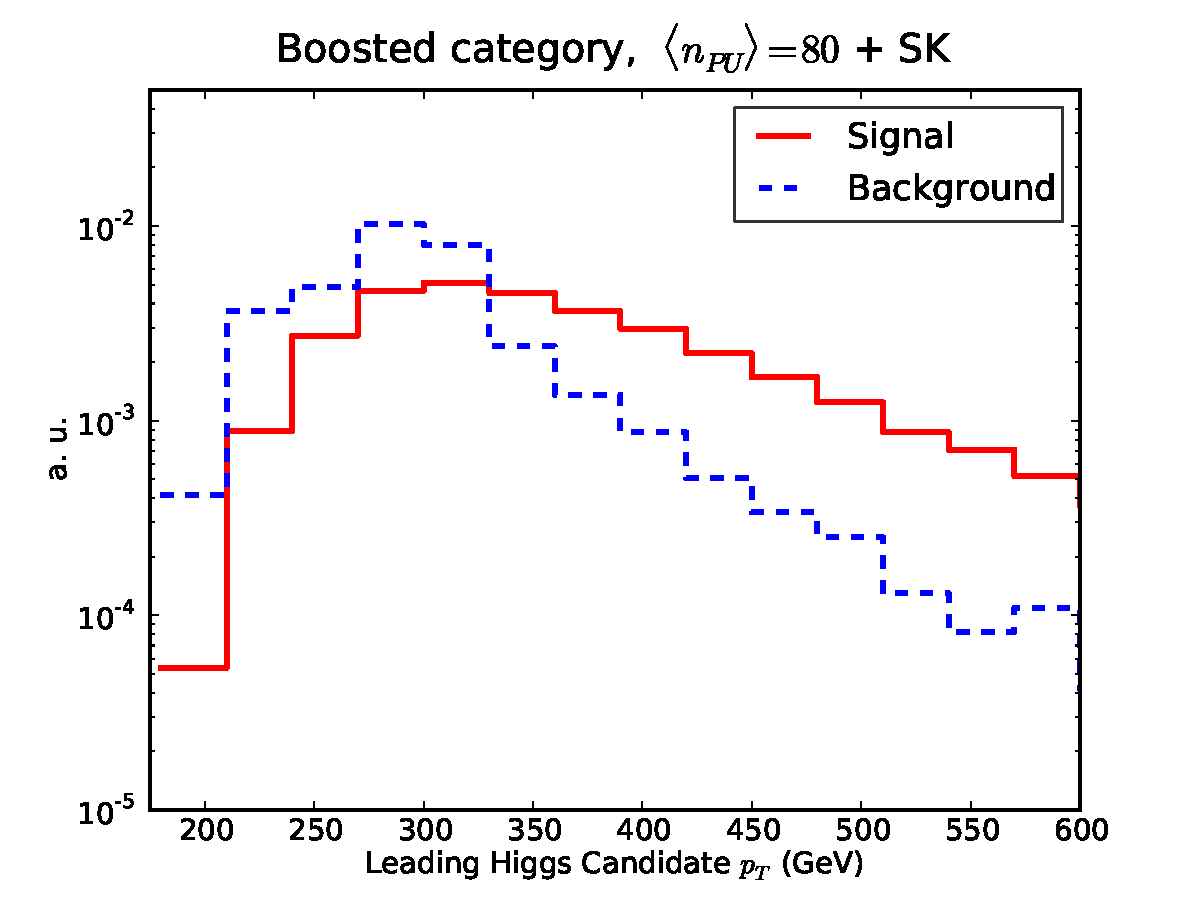
\includegraphics[width=0.49\textwidth]{plots/pt_h0_bst_comp_back.pdf}
   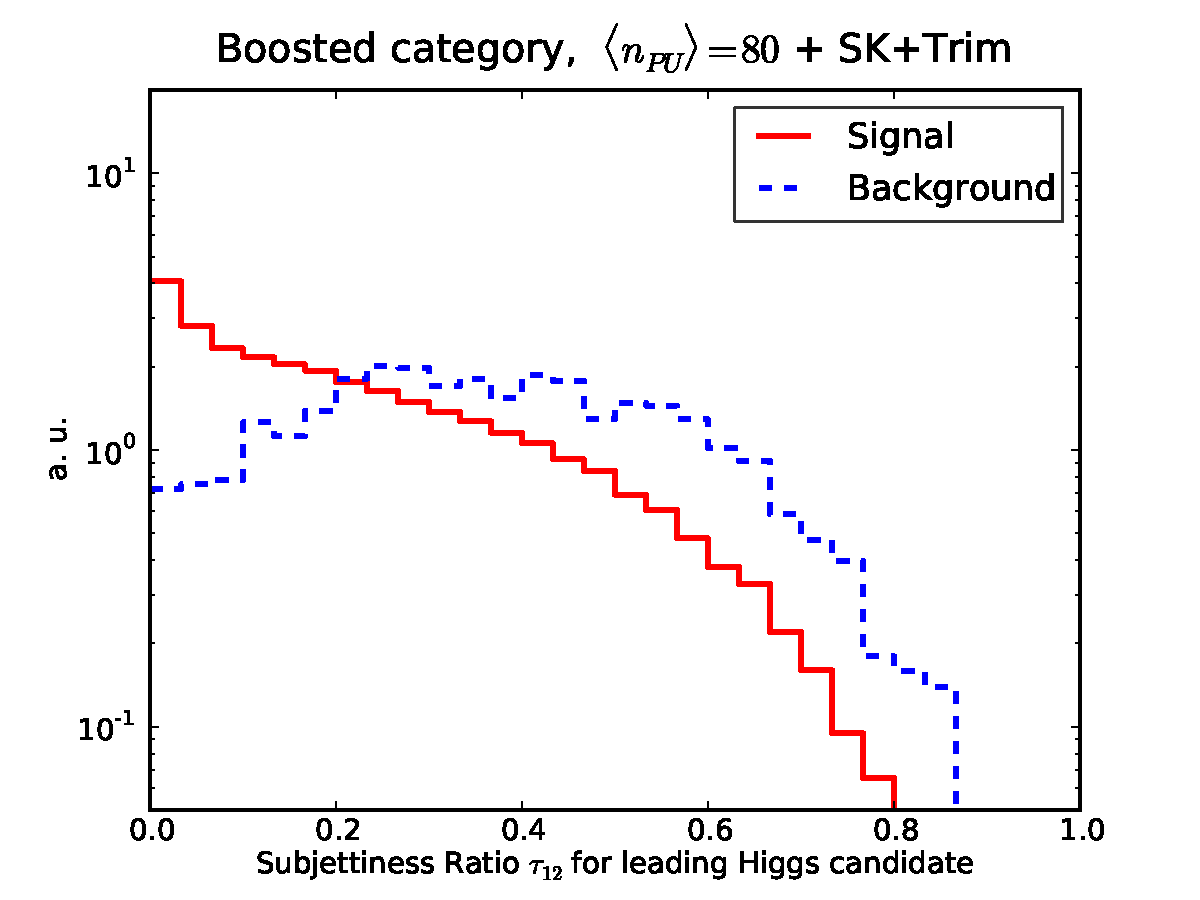
\includegraphics[width=0.49\textwidth]{plots/tau21_h1_bst_comp_back.pdf}
  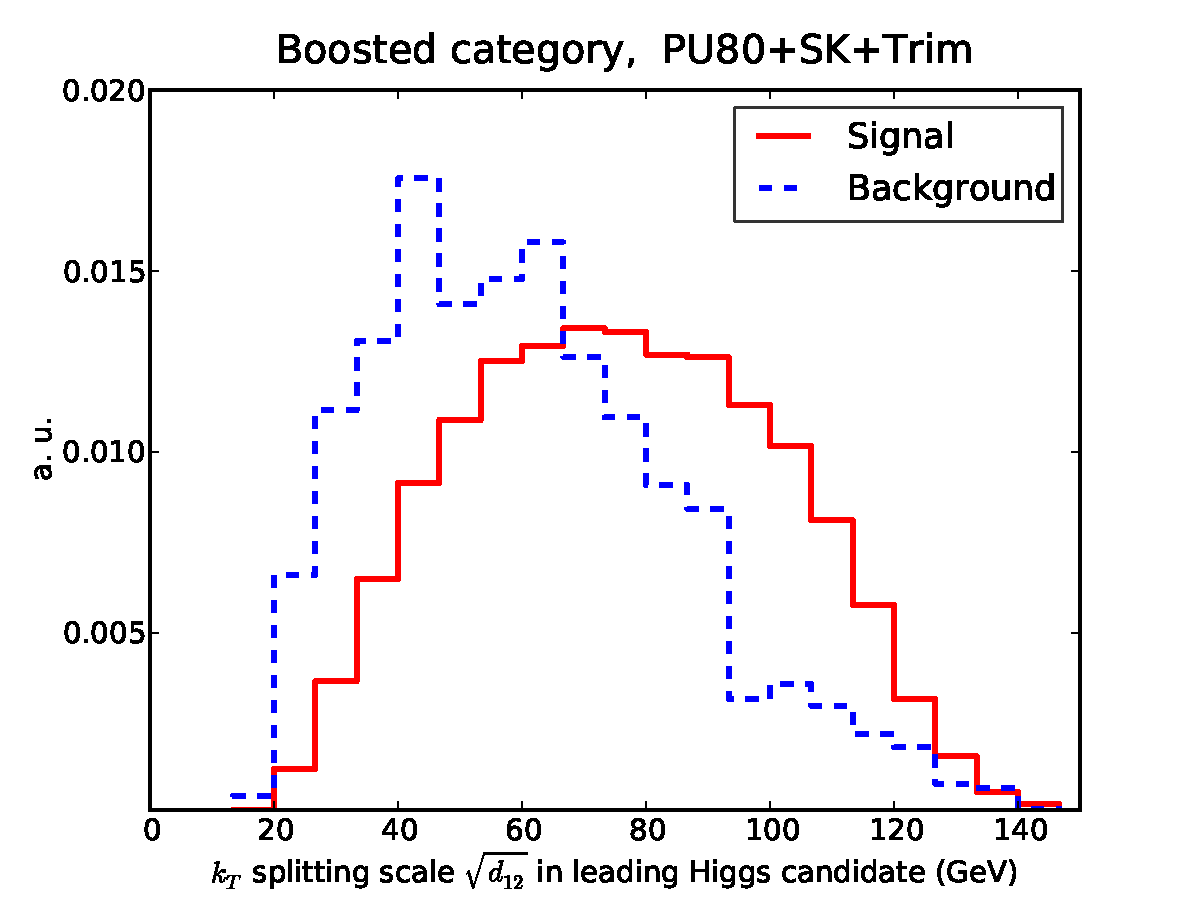
\includegraphics[width=0.49\textwidth]{plots/split12_h0_bst_comp_back.pdf}
   \caption{\small
     Comparison of kinematical distributions, in
     the boosted category, for signal and background events
     with and without PU: the invariant mass,  $p_T$,
     and the substructure variables $\tau_{21}$ and $\sqrt{d_{12}}$
    for the leading Higgs candidate.
     %
 }
\label{fig:signal-vs-back-boosted}
\end{center}
\end{figure}
%%%%%%%%%%%%%%%%%%%%%%%



Now we perform a similar comparison this time for
the resolved category.
%
In Fig.~\ref{fig:signal-vs-back-resolved} we compare
the kinematical distributions for signal and background events,
     with and without PU, for the invariant mass and the $p_T$ of the leading
     Higgs candidate.
     %
     Also in this
     case the PU-subtracted background distributions appear reasonably close
     to their no PU counterparts.
     %
     Therefore, these results
     suggest that the broad pattern of the signal over background
     discrimination provided by the MVA in Sect.~\ref{sec:mva},
     based on the corresponding differences between kinematical
     distributions,
will
     be maintained in the presence of PU.
     %
     In the next section we verify this expectation.


%%%%%%%%%%%%%%%%%%%%%%%%
\begin{figure}[t]
  \begin{center}
   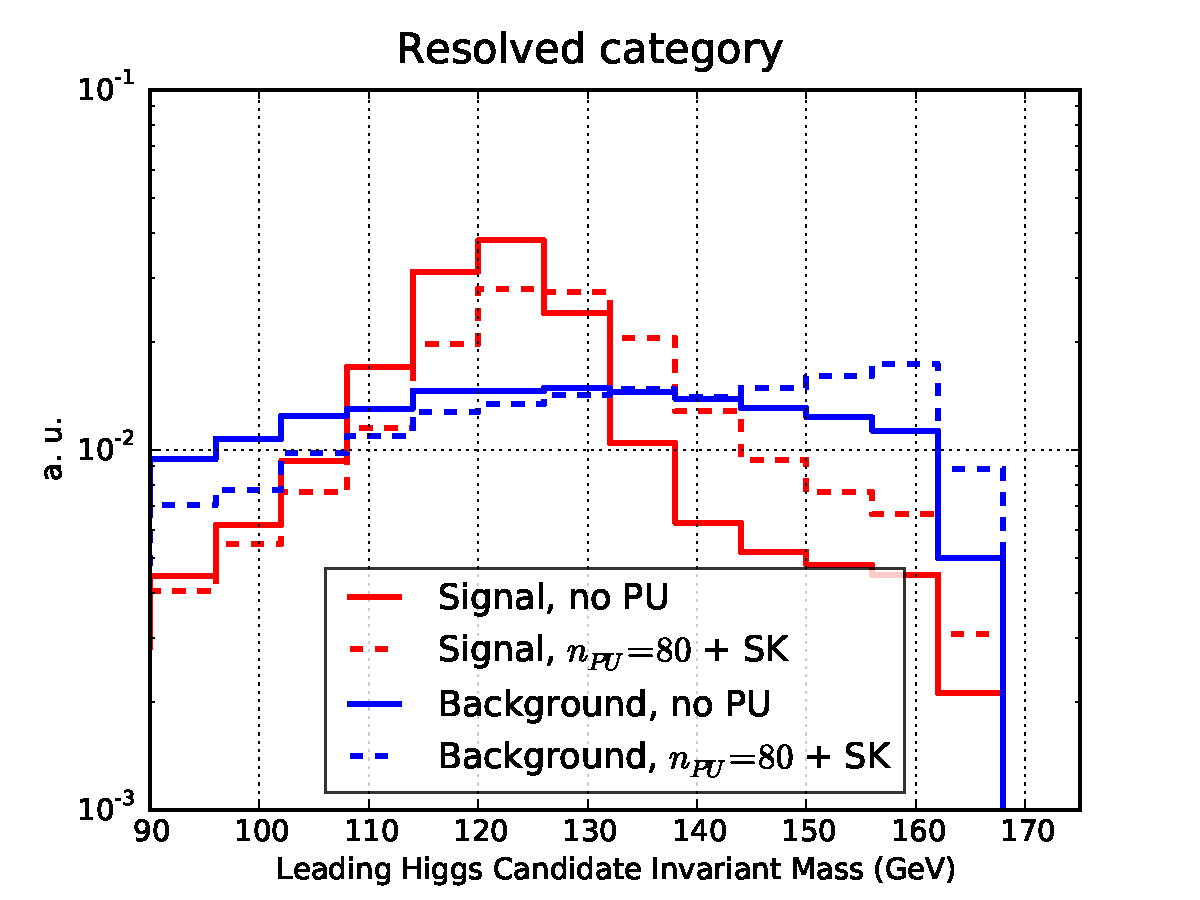
\includegraphics[width=0.49\textwidth]{plots/m_h0_res_comp_back.pdf}
  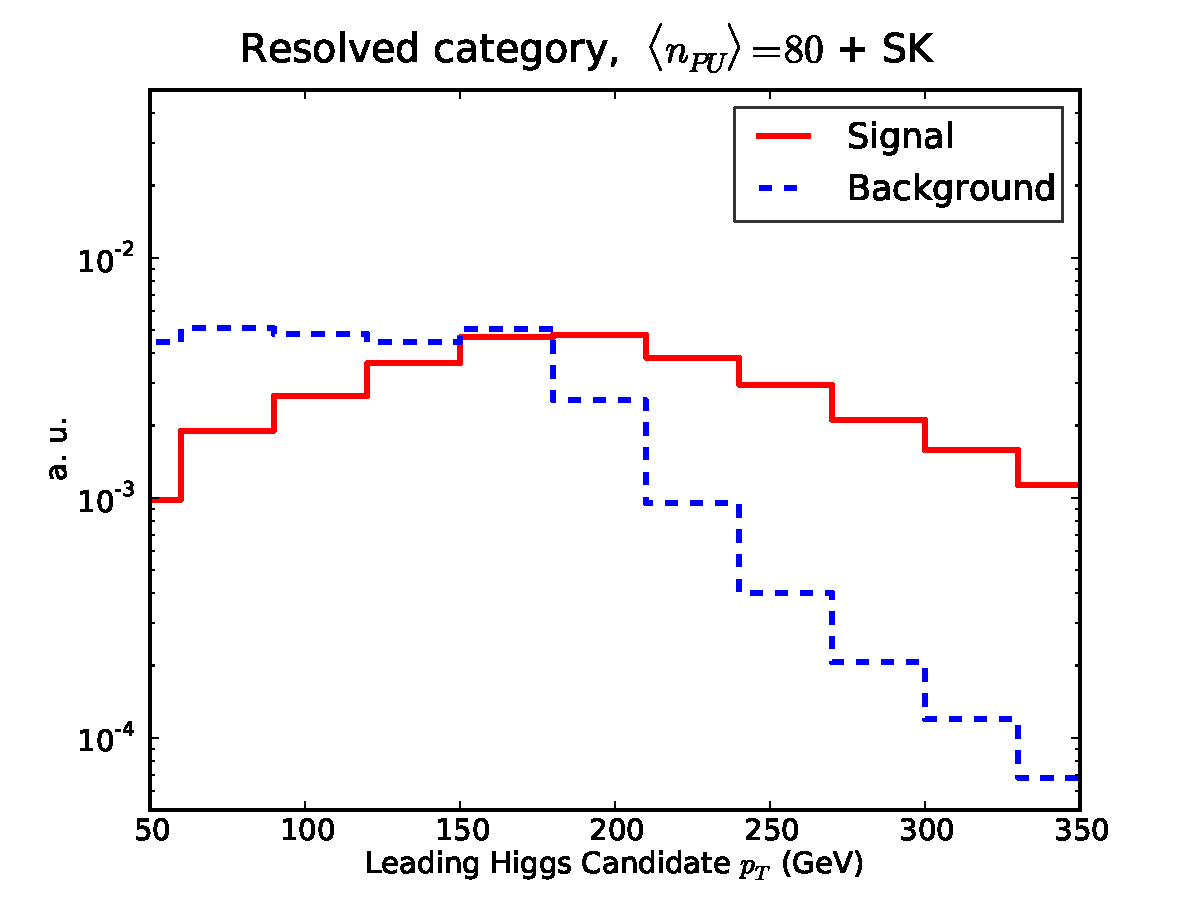
\includegraphics[width=0.49\textwidth]{plots/pt_h0_res_comp_back.pdf}
     \caption{\small
       Same as Fig.~\ref{fig:signal-vs-back-boosted} for the resolved category,
       this time without the jet substructure variables.
}
\label{fig:signal-vs-back-resolved}
\end{center}
\end{figure}
%%%%%%%%%%%%%%%%%%%%%%%

\subsection{MVA revisited in the presence of PU}

The same settings of the cut-based analysis,
Sects.~\ref{sec:analysis} and~\ref{sec:results}, and
the subsequent MVA optimization, Sect.~\ref{sec:mva}, have
been applied to the samples with PU, $\la n_{\rm PU}\ra=80$,
and SK subtraction.
%
The corresponding version of Table~\ref{tab:cutflow_noPU_1}, the 
cut-flow for the cross-sections and signal significance at the various
steps of the cut-based analysis, 
in the case
of PU subtracted with SK, for $\la n_{\rm PU}\ra=80$,
is presented in Table~\ref{tab:cutflow_SKPU80_1}.
%
One immediate observation is that
at the end of the cut-based analysis,
the signal significance have been  degraded
as compared to the case without PU.
%
We now obtain values for $S\sqrt{B}$ of 0.4, 0.3 and 0.9, in the resolved,
intermediate and boosted categories, respectively, to be compared
with the corresponding values without PU, namely 1.6, 1.6 and 2.7.
%
Therefore, the pre-MVA signal significance is degraded by a factor 4 in
the resolved and the intermediate categories,
and by a factor 3 in the boosted category.
%
The fact that the latter is the  least affected one
can be understood from the previous comparison
plots, which show that effects of PU contamination
are milder due to the  selection requirements
of the boosted category.

%%%%%%%%%%%%%%%%%%%%%%%%%%%%%%%%%%%%%%%%%%%%%%%%%%%%%%%%%%%
\begin{table}[t]
  \centering
  \scriptsize
  \begin{tabular}{|l|cc|cccc|cccc|}
  \hline
\multicolumn{11}{|c|}{Resolved category, $\la n_{\rm PU}\ra=80$+SK}\\
\hline
&  \multicolumn{6}{c|}{Cross-section [pb]} &  &  & &  \\
   &  $hh\to 4b$ &  total bkg  &   $4b$    &  $2b2j$   &   $4j$    &
$t\bar{t}$ &
$S/B_{\rm tot}$ & $S/B_{\rm 4b}$ & $S/\sqrt{B_{\rm tot}}$ & $S\sqrt{B_{\rm 4b}}$ \\
  \hline
  \hline
 C0    & 16  &   $3.1\cdot 10^9$   & $9.0\cdot 10^5$ & $2.1\cdot 10^8$ & $2.9\cdot 10^9$ & $1.8\cdot 10^5$ &   $5.0\cdot 10^{-9}$   & $1.7\cdot 10^{-5}$ &   $1.5\cdot 10^{-2}$   & 0.9 \\
 C1a   & 16  &   $3.1\cdot 10^9$   & $9.0\cdot 10^5$ & $2.1\cdot 10^8$ & $2.9\cdot 10^9$ & $1.8\cdot 10^5$ &   $5.0\cdot 10^{-9}$   & $1.7\cdot 10^{-5}$  &   $1.5\cdot 10^{-2}$   & 0.9 \\
 C1c   & 13  &   $1.1\cdot 10^9$   & $2.5\cdot 10^5$ & $7.7\cdot 10^7$ & $1.1\cdot 10^9$ & $1.3\cdot 10^5$ &   $1.1\cdot 10^{-8}$   & $5.3\cdot 10^{-5}$  &   $2.1\cdot 10^{-2}$   & 1.4  \\
 C1d   & 13 &   $1.1\cdot 10^9 $  & $2.5\cdot 10^5$ & $7.7\cdot 10^7$ & $1.1\cdot 10^9$ & $1.3\cdot 10^5$  &   $1.1\cdot 10^{-8}$   & $5.3\cdot 10^{-5}$  &   $2.1\cdot 10^{-2}$   & 1.4\\
 C1e   & 1.3  &   $3.9\cdot 10^7$   & $1.2\cdot 10^4$ & $2.8\cdot 10^6$ & $3.6\cdot 10^7$ & $3.3\cdot 10^4$  &   $3.4\cdot 10^{-8}$   & $1.1\cdot 10^{-4}$ &   $1.2\cdot 10^{-2}$   & 0.6\\
 C2    & 0.22  &   $2.3\cdot 10^3$   & $7.4\cdot 10^2$ & $1.4\cdot 10^3$ & $9.9\cdot 10^1$ & $1.6\cdot 10^1$  &   $9.8\cdot 10^{-5}$   & $3.0\cdot 10^{-4}$  &  $0.25$   & 0.4 \\
\hline
\end{tabular}

  $\,$ \\
  \vspace{0.5cm}
  \begin{tabular}{|l|cc|cccc|cccc|}
  \hline
\multicolumn{11}{|c|}{Intermediate category}\\
\hline
&  \multicolumn{6}{c|}{Cross-section [pb]} &  &  & &  \\
   &  $hh\to 4b$ &  total bkg  &   $4b$    &  $2b2j$   &   $4j$    &
$t\bar{t}$ &
$S/B_{\rm tot}$ & $S/B_{\rm 4b}$ & $S/\sqrt{B_{\rm tot}}$ & $S\sqrt{B_{\rm 4b}}$ \\
  \hline
  \hline
C0      & 16  &   $3.1\cdot 10^9$   & $9.0\cdot 10^5$ &  $2.1\cdot 10^8$ & $2.9\cdot 10^9$ & $1.8\cdot 10^5$ &   $5.0\cdot 10^{-9}$   & $1.7\cdot 10^{-5}$ &    $1.5\cdot 10^{-2}$   & 0.9\\
 C1b     & 6.1  &  $ 4.6\cdot 10^8$   &$ 1.6\cdot 10^5$ & $3.1\cdot 10^7$ & $4.3\cdot 10^8$ & $3.6\cdot 10^4$  &  $ 1.3\cdot 10^{-8}$   & $3.9\cdot 10^{-5}$  & $1.6\cdot 10^{-2}$   & 0.9 \\
 C1c     & 3.1  &   $8.7\cdot 10^7 $  & $2.4\cdot 10^4$ & $5.7\cdot 10^6$ & $8.1\cdot 10^7$ & $2.6\cdot 10^4$ &   $3.6\cdot 10^{-8}$   & $1.3\cdot 10^{-4}$ &  $1.8\cdot 10^{-2}$    & 1.1 \\ 
 C1d     & 3.2  &   $8.6\cdot 10^7 $  & $1.9\cdot 10^4$ & $5.6\cdot 10^6$ & $8.0\cdot 10^7$ & $2.4\cdot 10^4$  &   $3.7\cdot 10^{-8}$   & $1.7\cdot 10^{-4}$ &   $1.9\cdot 10^{-2}$   & 1.3 \\
 C1e     & 0.43  &   $2.7\cdot 10^7$   & $7.0\cdot 10^3$ & $1.8\cdot 10^6$ & $2.5\cdot 10^7$ & $9.3\cdot 10^3$  &   $1.6\cdot 10^{-8}$   & $6.2\cdot 10^{-5}$  &     $4.6\cdot 10^{-3}$   & 0.3 \\
 C2      & $3.2\cdot 10^{-2}$  &   $2.7\cdot 10^2$   & $3.7\cdot 10^1$ & $2.1\cdot 10^2$ & $1.8\cdot 10^1$ & 1.2 &  $ 1.2\cdot 10^{-4}$   & $8.6\cdot 10^{-4}$  &      0.1   & 0.3 \\
\hline
\end{tabular}

  $\,$ \\
  \vspace{0.5cm}
    \begin{tabular}{|l|cc|cccc|cccc|}
  \hline
\multicolumn{11}{|c|}{Boosted category, $\la n_{\rm PU}\ra=80$+SK}\\
\hline
&  \multicolumn{6}{c|}{Cross-section [pb]} &  &  & &  \\
   &  $hh\to 4b$ &  total bkg  &   $4b$    &  $2b2j$   &   $4j$    &
$t\bar{t}$ &
$S/B_{\rm tot}$ & $S/B_{\rm 4b}$ & $S/\sqrt{B_{\rm tot}}$ & $S\sqrt{B_{\rm 4b}}$ \\
  \hline
  \hline
 C0      & 16  &   $3.1\cdot 10^9$   & $9.0\cdot 10^5$ & $2.1\cdot 10^8$ & $2.9\cdot 10^9$ & $1.8\cdot 10^5$ &   $5.0\cdot 10^{-9}$   & $1.7\cdot 10^{-5}$  &   $1.5\cdot 10^{-2}$   & 0.9 \\
 C1a     & 16  &   $3.1\cdot 10^9 $  & $9.0\cdot 10^5$ & $2.1\cdot 10^8$ & $2.9\cdot 10^9$ & $1.8\cdot 10^5$ &   $5.0\cdot 10^{-9}$   & $1.7\cdot 10^{-5}$   &   $1.5\cdot 10^{-2}$   & 0.9 \\
 C1c     & 3.9  &   $4.7\cdot 10^8 $  & $8.9\cdot 10^3$ & $3.1\cdot 10^7$ & $4.3\cdot 10^8$ & $1.6\cdot 10^4$   &  $ 8.4\cdot 10^{-9}$   & $4.4\cdot 10^{-4}$  &  $ 9.9\cdot 10^{-3}$   & 2.3 \\
 C1d     & 2.7  &   $4.4\cdot 10^8 $  & $5.4\cdot 10^3$ & $2.9\cdot 10^7$ & $4.1\cdot 10^8$ & $1.3\cdot 10^4$ &   $6.0\cdot 10^{-9}$   & $5.0\cdot 10^{-4}$  &   $7.0\cdot 10^{-3}$   & 2.0 \\
 C1e     & 0.95  &   $1.1\cdot 10^7$   & $1.5\cdot 10^3$ & $7.0\cdot 10^5$ & $9.8\cdot 10^6$ & $4.7\cdot 10^3$  &  $ 9.1\cdot 10^{-8}$   & $6.4\cdot 10^{-4}$  &   $1.6\cdot 10^{-2}$   & 1.4 \\
 C2      & 0.11  &   $2.7\cdot 10^2$   & $4.2\cdot 10^1$ & $2.1\cdot 10^2$ & $1.1\cdot 10^1$ & $6.8\cdot 10^{-1}$  &  $ 4.0\cdot 10^{-4}$   & $2.5\cdot 10^{-3}$  &   $0.35$   & 0.9 \\
\hline
\end{tabular}

    \caption{\small
      Same as Table~\ref{tab:cutflow_noPU_1}, for the analysis
      including PU with $\la n_{\rm PU}\ra=80$ and SK subtraction.
      \label{tab:cutflow_SKPU80_1}}
\end{table}
%%%%%%%%%%%%%%%%%%%%%%%%%%%%%%%%%%%%%%%%%%%%%%%%%%%%%%%%%%


In Fig.~\ref{fig:nnresponse_PU} we present
the distribution of the ANN output for the
signal and background MC events in the boosted and resolved categories --
the analogous comparison in the case without PU was shown
in Fig.~\ref{fig:nnresponse}.
%
We observe that the clear MVA discrimination
between signal and background events in the two categories is robust
when PU is included.
%
However, by comparing with Fig.~\ref{fig:nnresponse}, we see
that some of the most distinguishing features that separate signal
and background in the ANN output are reduced when PU effects
are included.
%
For instance, in the boosted category, there is a trend of the distribution
for signal events to move towards smaller values of the
ANN discriminant.
%
This in turn will entail a reduction of the signal significance as
compared to the case without PU.

%%%%%%%%%%%%%%%%%%%%%%%%%%%%
\begin{figure}[t]
  \begin{center}
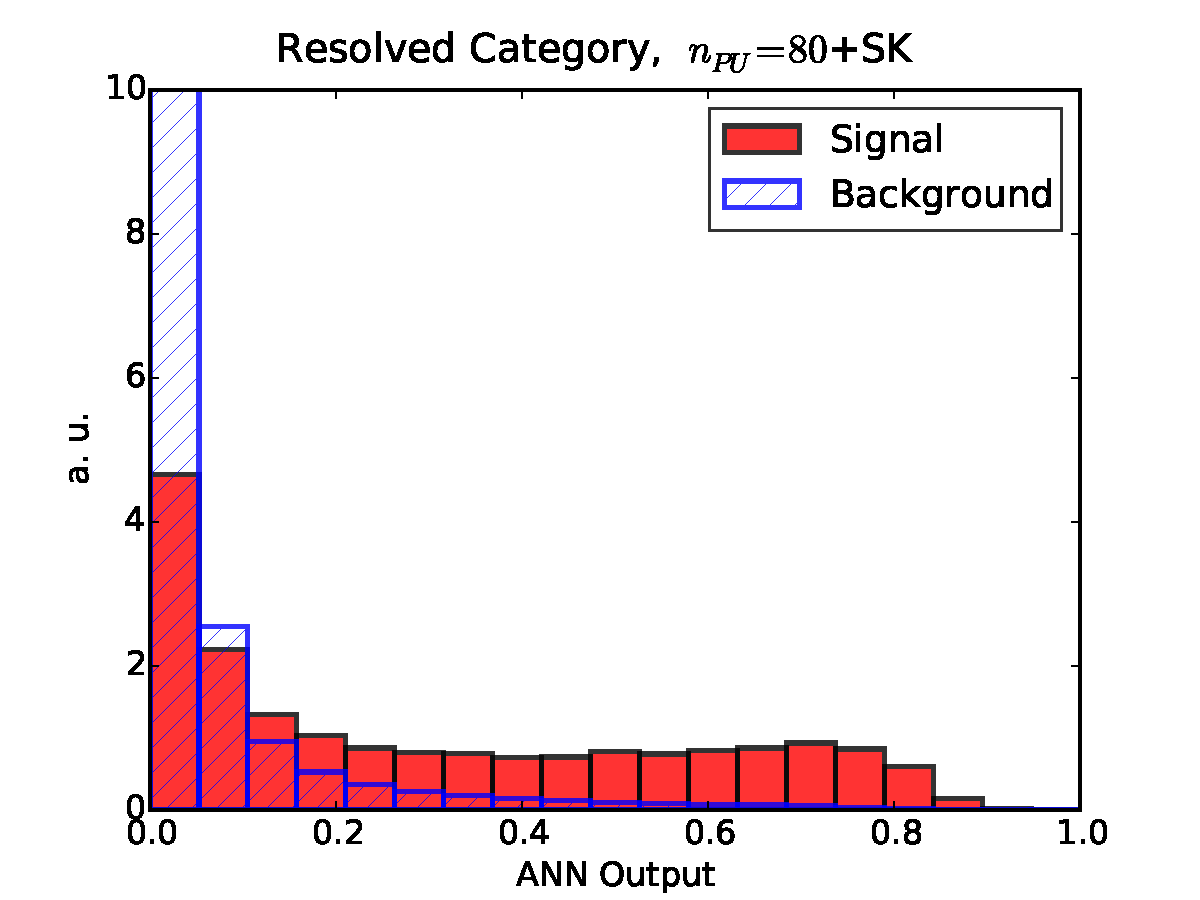
\includegraphics[width=0.49\textwidth]{plots/Resolved_disc_SKPU80.pdf}
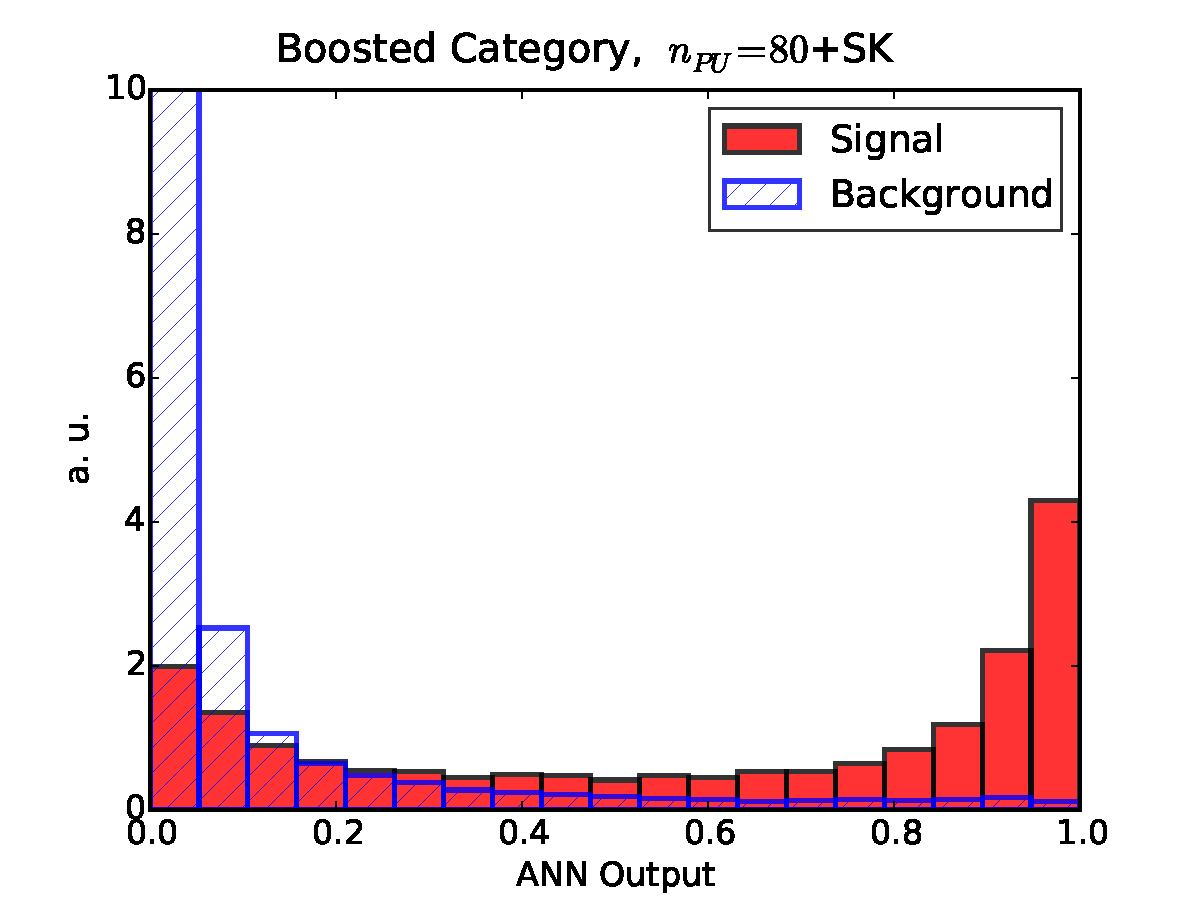
\includegraphics[width=0.49\textwidth]{plots/Boosted_disc_SKPU80.pdf}
\caption{\small Same as Fig.~\ref{fig:nnresponse},
  this time with $\la n_{\rm PU}\ra=80$ PU events per bunch crossing
  and SK subtraction, for the resolved (left) and boosted
  (right) categories.
  %
  The corresponding comparison without PU was shown in
  Fig.~\ref{fig:nnresponse}.
}
\label{fig:nnresponse_PU}
\end{center}
\end{figure}
%%%%%%%%%%%%%%%%%%%%%%%


In Table~\ref{table:cutflowMVA_PU}
we provide the  the number of signal and
    background events expected
    at the HL-LHC, as well as the
    corresponding values for $S/\sqrt{B}$ and $S/B$,
    for both the cut-based analysis (corresponding
    to $y_{\rm cut}=0$) and after the
    optimal MVA cut, for the simulations
    with $\la n_{\rm PU}\ra=80$
    and SK subtraction.
    %
    The same results without PU are those of
    Table.~\ref{table:cutflowMVA}.
    %
    From Table~\ref{table:cutflowMVA_PU} we see that, thanks
to the MVA, we can improve the signal significance and the
signal over background ratio from 0.35 and $4\cdot 10^{-4}$
(0.25 and $1\cdot 10^{-4}$) up to 2.9 and 0.034 (2.5 and 0.15)
in the boosted (resolved) category.
%
The intermediate category exhibits a rather lower value of $S/\sqrt{B}$
for the optimal $y_{\rm cut}$ value, around 1.1.
%
We thus conclude that, as was already the case
without PU,
the boosted category is the most promising
one for the study of Higgs pair production in the $b\bar{b}b\bar{b}$
final state
at the HL-LHC, also when PU is included.
%
However, important information will also be obtained from
the resolved category, which has a signal significance
only slightly smaller than the boosted case.


%%%%%%%%%%%%%%%%%%%%%%%%%%%%%%%%%%%%%%%%%%%%%%%%%%%%%
\begin{table}[t]
  \centering
  \small
  \begin{tabular}{c|c|c|c||c|c|c|c}
    \hline
    \multicolumn{8}{c}{Boosted category, $\la n_{\rm PU}\ra=80$+SK}\\
    \hline
     \multicolumn{4}{c||}{no MVA cut} & \multicolumn{4}{c}{optimal MVA cut}\\
    \multicolumn{4}{c||}{$y_{\rm cut}=0$} & \multicolumn{4}{c}{$y_{\rm cut}=0.84$}\\
    \hline
    \multicolumn{2}{c|}{$N_{\rm ev}$} &  $S/\sqrt{B}$  & $S/B$
    & \multicolumn{2}{c|}{$N_{\rm ev}$} &  $S/\sqrt{B}$  & $S/B$\\
        Signal & Back   &     &   &  Signal & Back   &     &    \\
    \hline
    362  &  $1.4\cdot 10^6$     & 0.31       &  $3\cdot 10^{-4}$ &
    248     &   7250             &  2.9       & 0.034 \\
    \hline
       \multicolumn{8}{c}{$\quad$}\\
    \hline
    \multicolumn{8}{c}{Intermediate category,  $\la n_{\rm PU}\ra=80$+SK}\\
    \hline
    \multicolumn{4}{c||}{no MVA cut} & \multicolumn{4}{c}{optimal MVA cut}\\
    \multicolumn{4}{c||}{$y_{\rm cut}=0$} & \multicolumn{4}{c}{$y_{\rm cut}=0.72$}\\
    \hline
    \multicolumn{2}{c|}{$N_{\rm ev}$} &  $S/\sqrt{B}$  & $S/B$
    & \multicolumn{2}{c|}{$N_{\rm ev}$} &  $S/\sqrt{B}$  & $S/B$\\
        Signal & Back   &     &   &  Signal & Back   &     &    \\
    \hline
    146  &    $9\cdot 10^5$   & 0.15        &  $2\cdot 10^{-4}$      &
  53  &  2547        & 1.1        &  0.02 \\
  \hline
  \multicolumn{8}{c}{$\quad$}\\
    \hline
    \multicolumn{8}{c}{Resolved category,  $\la n_{\rm PU}\ra=80$+SK}\\
    \hline
     \multicolumn{4}{c||}{no MVA cut} & \multicolumn{4}{c}{optimal MVA cut}\\
    \multicolumn{4}{c||}{$y_{\rm cut}=0$} & \multicolumn{4}{c}{$y_{\rm cut}=0.49$}\\
    \hline
    \multicolumn{2}{c|}{$N_{\rm ev}$} &  $S/\sqrt{B}$  & $S/B$
    & \multicolumn{2}{c|}{$N_{\rm ev}$} &  $S/\sqrt{B}$  & $S/B$\\
        Signal & Back   &     &   &  Signal & Back   &     &    \\
    \hline
  1123  &    $8.5\cdot 10^6$   & 0.25       &  $1.3\cdot 10^{-4}$       &
  432  &  $3\cdot 10^4$        &   2.5      & 0.15 \\
        \hline
  \end{tabular}
  \caption{\small Same as Table~\ref{table:cutflowMVA} in the case
    of PU+SK, with $\la n_{\rm PU}\ra=80$.
        \label{table:cutflowMVA_PU}
  }
\end{table}
%%%%%%%%%%%%%%%%%%%%%%%%%%%%%%%%%%%%%%%%%%%%%%%%%%%%%

Another important result from Table~\ref{table:cutflowMVA_PU} is that,
for the optimal MVA cut, the signal over background ratio
is not unfeasibly small: we obtain that $S/B$ is 3.4\% (1.5\%)
in the boosted (resolved) categories.
%
This is indicates that while this measurement is still very challenging,
requiring a careful extraction from the data of the QCD
background, it is certainty within reach.
%
Our analysis also indicates a possible way forward to
further increase $S/B$: reducing the background from light and charm
fakes, see Table~\ref{tab:cutflow_SKPU80_1}.

Let us now discuss in more detail the results of the MVA
classification, by showing various estimators as function
of the cut $y_{\rm cut}$ in the ANN discriminant.
%
In Fig.~\ref{fig:nev2_PU}
we show the number of signal and background events that
are expected at the HL-LHC as a function of
$y_{\rm cut}$ -
the corresponding results without PU are those of
Fig.~\ref{fig:nev2}.
%
As we can see, the general trends are
similar as those without PU.
%
Comparing Figs.~\ref{fig:nev2} and~\ref{fig:nev2_PU}, we also observe
that the intermediate category is substantially degraded once PU effects
are accounted for, the reason being  sizable
a reduction in the number of signal
events that are now assigned to this category.
%
This shows that the selection criteria
of the intermediate category are less
resilient against PU contamination,
as opposed to the resolved and boosted selections.

%%%%%%%%%%%%%%%%%%%%%%%%%%%%%%%%%%%%%%%%%%%%%
\begin{figure}[t]
\begin{center}
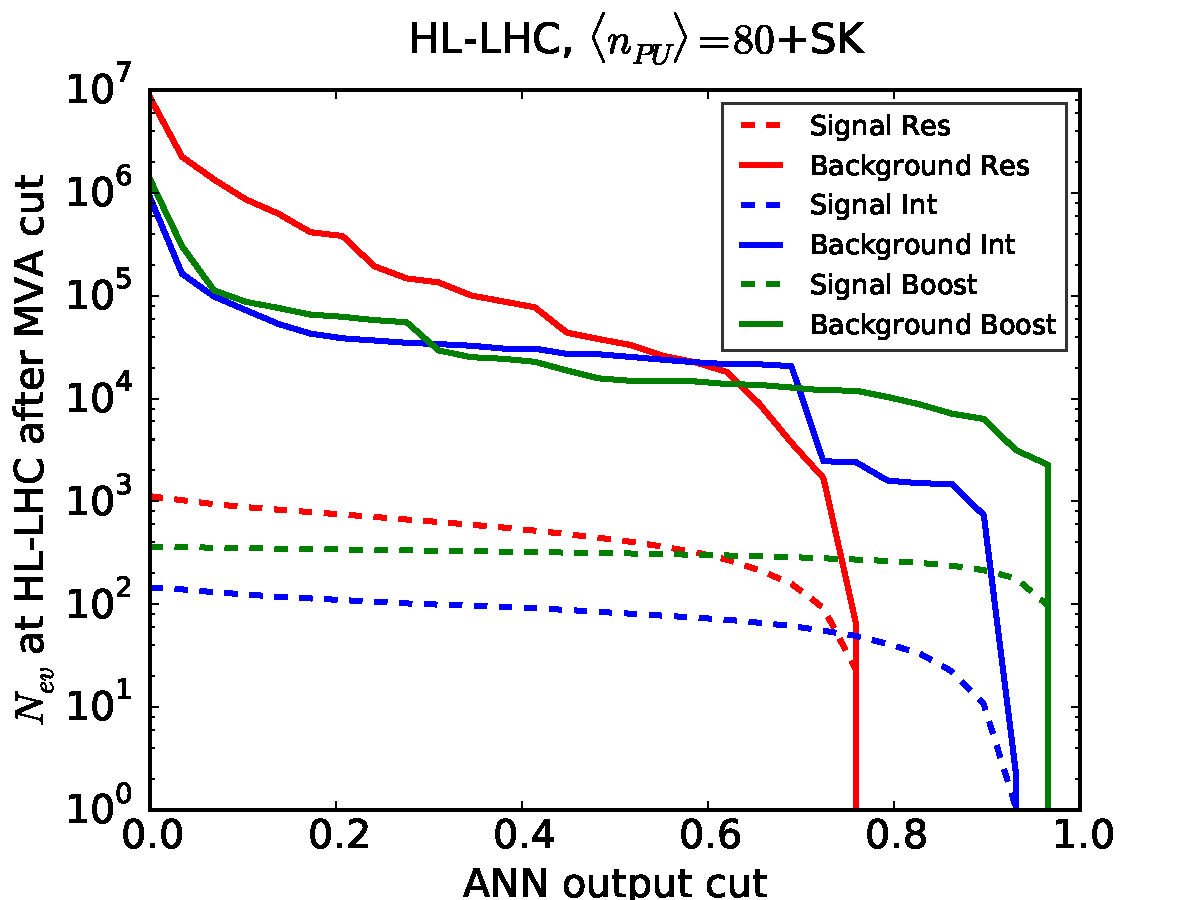
\includegraphics[width=0.65\textwidth]{plots/nev2_SKPU80.pdf}
\caption{\small Same as Fig.~\ref{fig:nev2} in the
case of events with PU, for
 $\la n_{\rm PU}\ra=80$ 
  and SK subtraction.
}
\label{fig:nev2_PU}
\end{center}
\end{figure}
%%%%%%%%%%%%%%%%%%%%%%%%%%%%%%%%%%%%%


In Fig.~\ref{fig:sb_mva_PU} we show the signal significance,
$S/\sqrt{B}$, as well as the signal over background ratio,
$S/B$, including now the effects of PU.
%
The corresponding results in the case without PU were shown in
Fig.~\ref{fig:sb_mva}.
%
As can be seen, the MVA-driven enhancement is robust in the
presence of PU.
%
While unsurprisingly there us a degradation as compared to the case wo PU,
we still manage to achieve a signal significance of
around $S/\sqrt{B}\simeq 2.5$ separately for the boosted and resolved
categories.
%
On the other hand, the intermediate category becomes irrelevant.
%
We conclude that the qualitative conclusions drawn in
Sect.~\ref{sec:mva} are robust in the presence
of realistic PU effects.
%
Since no specific effort has been performed to
optimize PU subtraction, for example by tuning the value
of the patch length $a$ in {\tt SoftKiller}, we believe that
there is
still room for improvement in this respect.


%%%%%%%%%%%%%%%%%%%%%%%%%%%%%%%%%%%%%%%%%%%%%%%%%%%%
%%%%%%%%%%%%%%%%%%%%%%%%%%%%%%%%%%%%%%%%%%%%%%%%%%%%
\begin{figure}[t]
\begin{center}
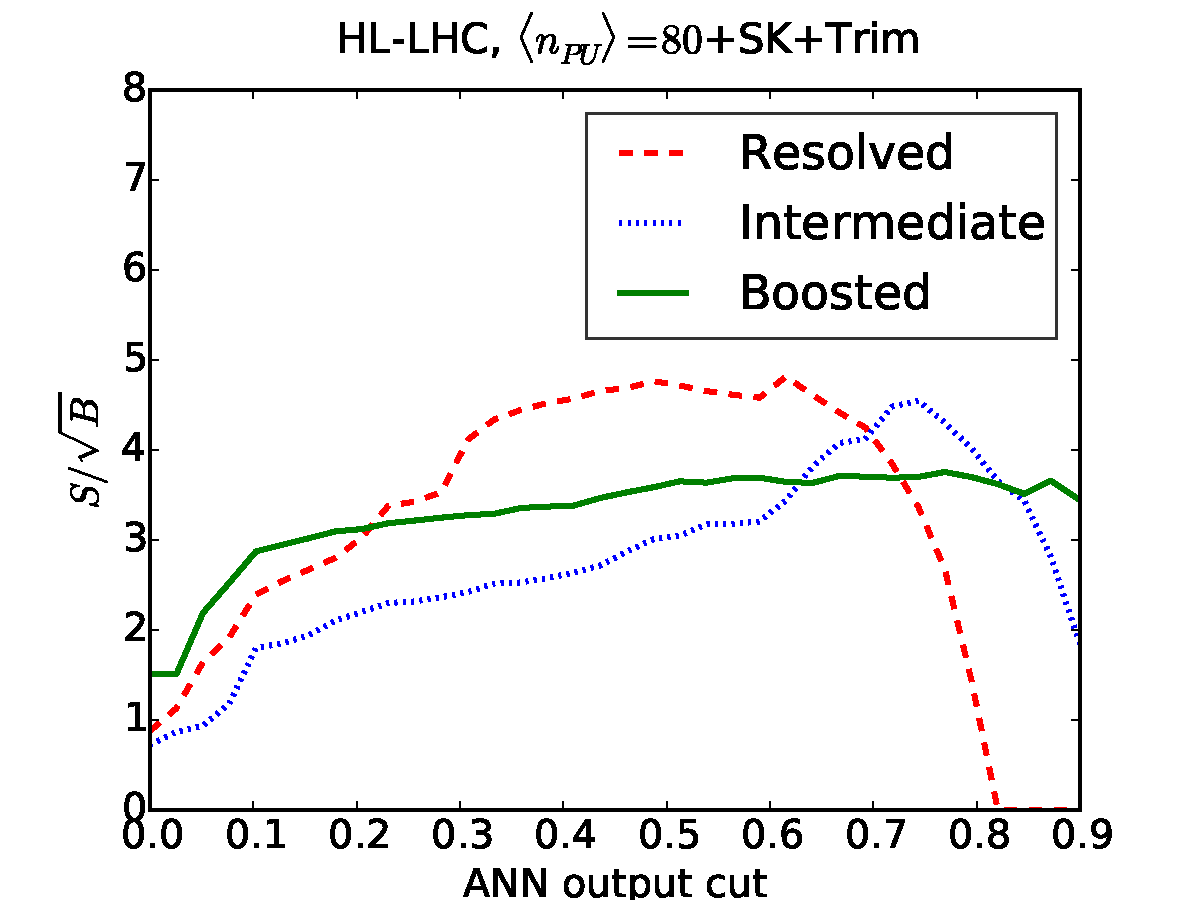
\includegraphics[width=0.48\textwidth]{plots/ssb_SKPU80.pdf}
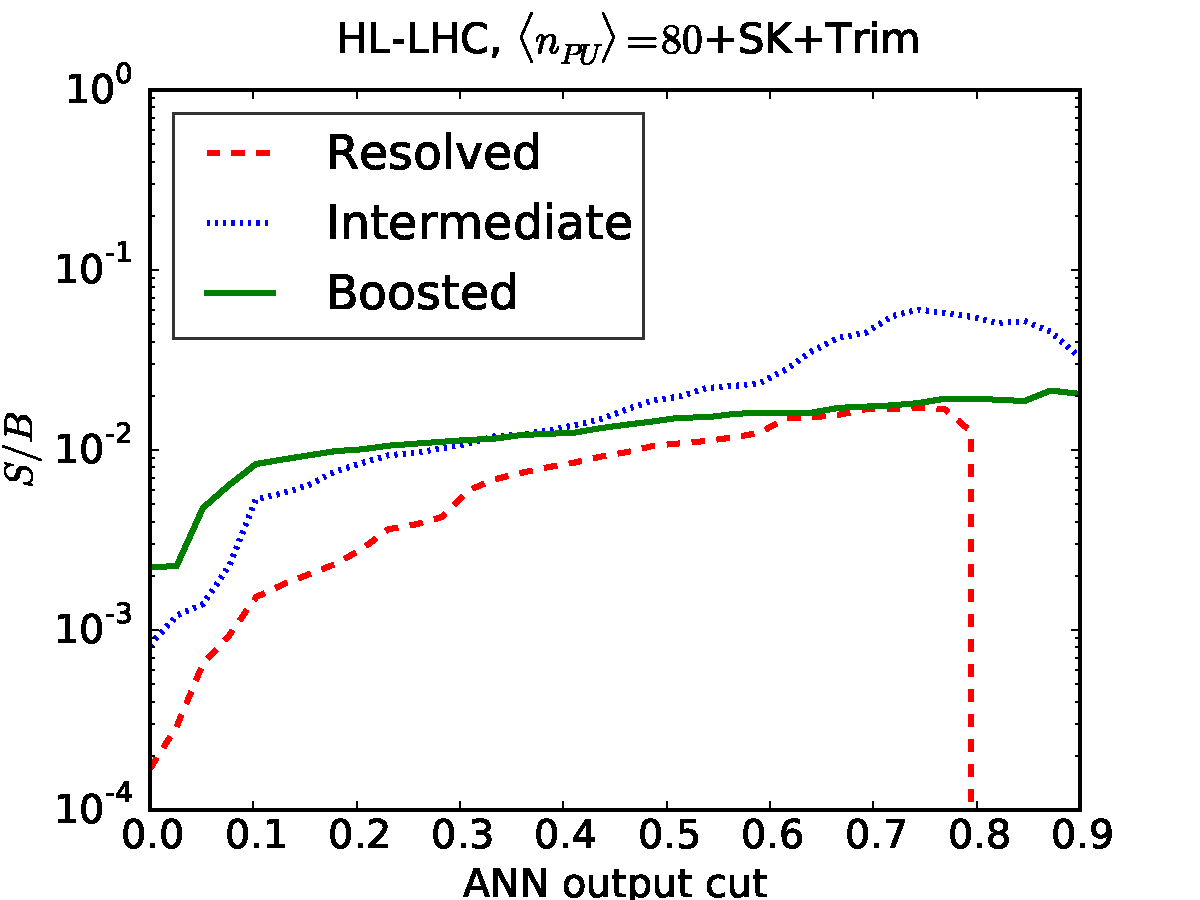
\includegraphics[width=0.48\textwidth]{plots/sb_SKPU80.pdf}
\caption{\small 
Same as Fig.~\ref{fig:sb_mva} in the
case of events with PU, for
 $\la n_{\rm PU}\ra=80$ 
  and SK subtraction.
}
\label{fig:sb_mva_PU}
\end{center}
\end{figure}
%%%%%%%%%%%%%%%%%%%%%%%

It is important to quantify which of the input variables
to the MVA carry the highest discrimination power
in the case of PU,
and compare it with the corresponding
results without PU.
%
We use the same estimator as in Sect.~\ref{sec:signalsignificance},
namely the sum
of the absolute value of all the weights connected to a given
input neuron $i$, Eq.~(\ref{eq:totweight}).
%
The results for the resolved and boosted categories are shown
on Fig.~\ref{fig:nnweights_PU}.
%
As we can see by comparing to the corresponding
results without PU in Fig.~\ref{fig:nnweights}, 
in the boosted category, the discrimination power of the invariant
mass of Higgs candidates is decreased and that of the various substructure
variables, in particular $C_2^{(\beta)}$ and
$D^{(\beta)}$, is conversely
increased.
%
This reflects the fact that these substructure variables are
relatively robust against PU contamination.
%
In addition, also the $p_T$ distributions of the AK03
subjets within the large-$R$
jets carry important information.
%
In the case of the resolved category,  the highest
values of the ANN weights without PU
were found for the $p_T$ of the leading
Higgs and for the Higgs invariant masses.
%
This is also true in the case with PU, but now the rapidity difference
between the two Higgs candidates, $\Delta y_{hh}$ increases its
importance, again reflecting that this variable is relatively
insensitive to PU effects.
%

%%%%%%%%%%%%%%%%%%%%%%%%
\begin{figure}[t]
\begin{center}
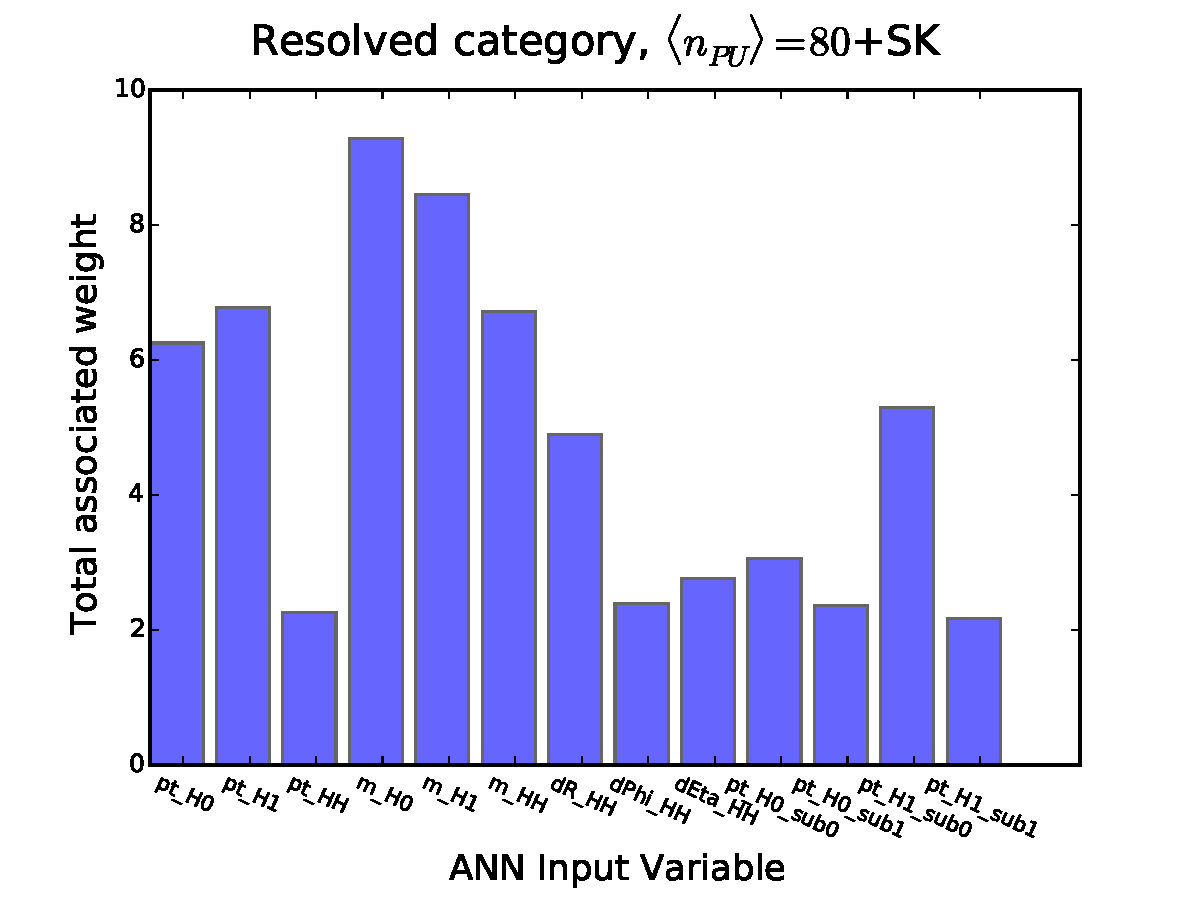
\includegraphics[width=0.49\textwidth]{plots/res_wgthist_SKPU80.pdf}
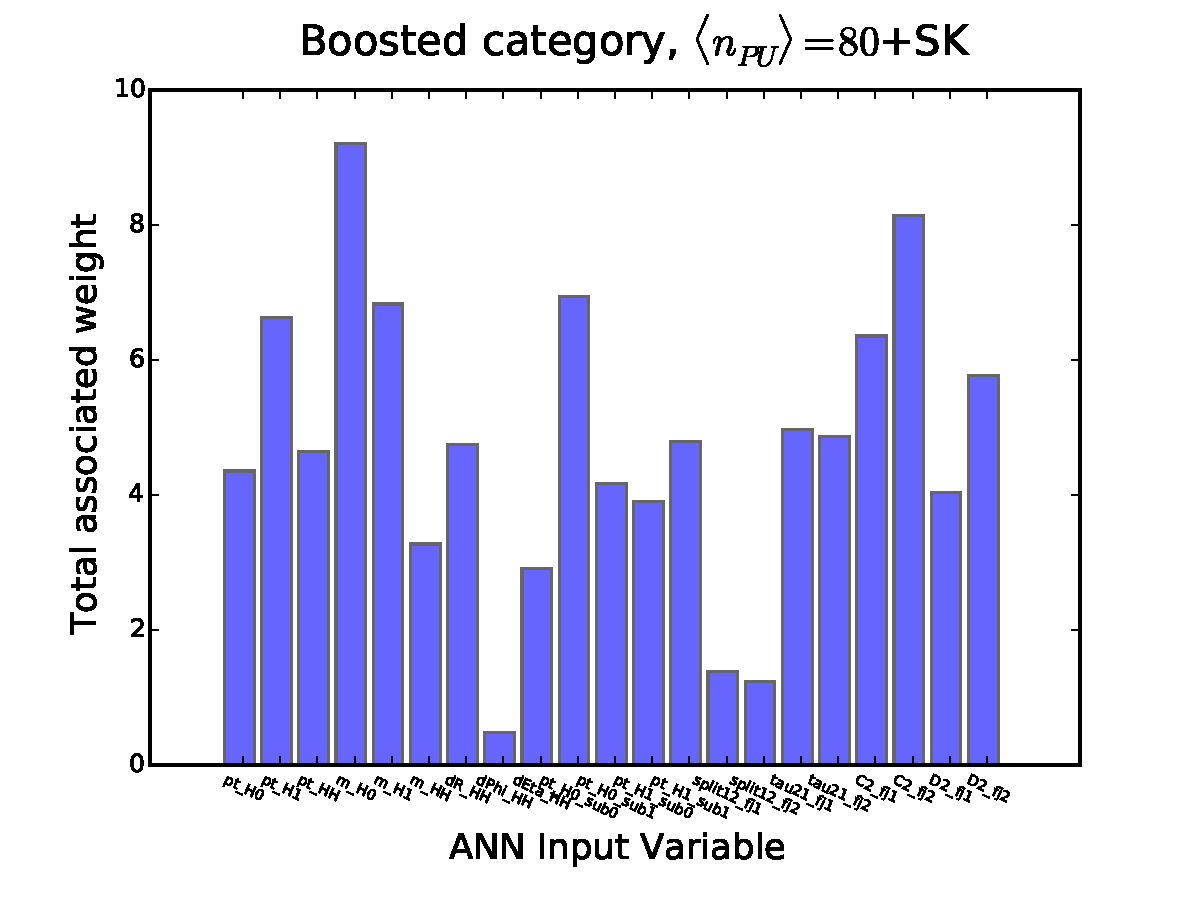
\includegraphics[width=0.49\textwidth]{plots/bst_wgthist_SKPU80.pdf}
\vspace{-0.5cm}
\caption{\small
Same as Fig.~\ref{fig:nnweights} in the
case of events with PU, for
 $\la n_{\rm PU}\ra=80$ 
  and SK subtraction.
}
\label{fig:nnweights_PU}
\end{center}
\end{figure}
%%%%%%%%%%%%%%%%%%%%%%%

At this point, we can finally combine the three categories, resolved,
intermediate and boosted, and determine the overall signal
significance taking into account all event topologies.
%
Adding in quadrature the signal significance from the three
(exclusive) categories for the corresponding
optimal value of $y_{\rm cut}$, our final combined result, accounting
for PU effects, is
\be
\lp \frac{S}{\sqrt{B}}\rp_{\rm tot} \simeq 4.0 \, ,
\ee
to be compared to the value $\lp S/\sqrt{B}\rp_{\rm tot} \simeq 8.5$
that was obtained in the case without PU.
%
We conclude that, even when realistic PU effects are accounted
for, at the HL-LHC the measurement of
Higgs pair production in the $b\bar{b}b\bar{b}$ final state should be 
well the threshold for evidence, and even meeting the
requirement for discovery might be within reach.
%

In summary, in this section we have demonstrated the robustness
of our results under the presence of PU conditions as those
expected at the HL-LHC.
%
With a signal significance of $S/\sqrt{B}\sim 4$, is clear that
the $b\bar{b}b\bar{b}$ final state can be used to claim evidence
for Higgs pair production at the HL-LHC without the need
to combine with any other final state.
%
Our analysis certainly contains
room for improvement, in particular by means of a tailored
study dedicated to optimize PU subtraction in this process.
%
It will be important now to quantify the precision of
a extraction of the Higgs trilinear coupling $\lambda$ using
the techniques presented here, but this is left for future work.

%%%%%%%%%%%%%%%%%%%%%%%%%%%%%%%%%%%%%%%%%%%%%%%%%%%%%%%%%%%%%%%%%%%%%%%%%%%%%%%%
%%%%%%%%%%%%%%%%%%%%%%%%%%%%%%%%%%%%%%%%%%%%%%%%%%%%%%%%%%%%%%%%%%%%%%%%%%%%%%%%
%%%%%%%%%%%%%%%%%%%%%%%%%%%%%%%%%%%%%%%%%%%%%%%%%%%%%%%%%%%%%%%%%%%%%%%%%%%%%%%%
%%%%%%%%%%%%%%%%%%%%%%%%%%%%%%%%%%%%%%%%%%%%%%%%%%%%%%%%%%%%%%%%%%%%%%%%%%%%%%%%
%%%%%%%%%%%%%%%%%%%%%%%%%%%%%%%%%%%%%%%%%%%%%%%%%%%%%%%%%%%%%%%%%%%%%%%%%%%%%%%%
